\documentclass{article}
\usepackage[margin=0.5in,bottom=1in,top=1in]{geometry}
%Attempt to make changes and see if git registers.
% header formatting
\usepackage{fancyhdr}

% For drawing chemical structures 
\usepackage{chemfig}
\usepackage{xcolor}
\usepackage{twoopt}
\usepackage{ifmtarg}

\usepackage{gensymb}
 
\pagestyle{fancy}
\fancyhf{}
\fancyhead[LE,RO]{Michael Yao}
\fancyhead[RE,LO]{MCAT Study Guide, SU2019}
\fancyfoot[CE,CO]{\leftmark}
\fancyfoot[LE,RO]{\thepage}

\renewcommand{\headrulewidth}{0.75pt}
\renewcommand{\footrulewidth}{0.75pt}

\usepackage[version=4]{mhchem}
\def\ZZ#1{\global\setbondstyle{thick,color=#1}\gdef\printatom##1{\color{#1}\ensuremath{\mathrm{##1}}}}
\def\paren#1{\rlap{\kern-.75em$\left(\vrule height1ex width0pt depth1ex\vrule height0pt width2.5em depth0pt\right)_{\!#1}$}}
\definesubmol\NN{-[,,,,draw=none]}
% atom numbers (used when option atom-numbers is selected)
\newcommand{\mcfatomno}[1]{\raisebox{2pt}{\color{blue}{\ensuremath{\mathsf{_{#1}}}}}}
\definesubmol\Red{(!\NN\ZZ{red})}
\definesubmol\Green{(!\NN\ZZ{green!40!black})}
\definesubmol\Purple{(!\NN\ZZ{purple})}
\definesubmol\Black{(!\NN\ZZ{black})}
%\setatomsep{2em}\setbondstyle{thick}

% math packages
\usepackage{mathtools}
\usepackage{amsmath}
\usepackage{amssymb}    % Math symbols such as \mathbb
\newcommand{\dbar}{{\mathchar '26\mkern -12mud}}
\usepackage{bbm}
\usepackage{gensymb}
\usepackage{amsthm}
\usepackage{pgfplots}   % plots
\usepackage{pbsi}
\usepackage[T1]{fontenc}

% other packages
\usepackage{graphicx}
\graphicspath{ {../assets/} }
\usepackage{enumitem}
\usepackage{color}
\usepackage{hyperref}
\hypersetup{
    colorlinks=true,
    linktoc=all,     %set to all if you want both sections and subsections linked
    linkcolor=blue,
}

% proper inline math display, adjust height for symbols like \sum
\everymath{\displaystyle}

% define tags for math use..
\theoremstyle{plain}% default
\newtheorem{theorem}{Theorem}[section]
\newtheorem{corollary}{Corollary}[theorem]

\theoremstyle{definition}
\newtheorem{defn}{Definition}[section]
\newtheorem{proposition}{Proposition}[defn]
\newtheorem{exmp}{Example}[section]

\theoremstyle{remark}
\newtheorem*{rem}{Remark}
\newtheorem*{note}{Note}
\newtheorem{case}{Case}

% Gives begin{solution} same formating as \begin{proof}
\newenvironment{solution}
  {\begin{proof}[Solution]}
  {\end{proof}}


%running fraction with slash - requires math mode.
\newcommand*\rfrac[2]{{}^{#1}\!/_{#2}}
%shortcut to mathbb
\newcommand{\N}{\mathbb{N}}
\newcommand{\R}{\mathbb{R}}
\newcommand{\C}{\mathbb{C}}
% color highlighting
\newcommand{\hilight}[1]{\colorbox{yellow}{#1}}

\title{\vspace{-6ex}MCAT Study Guide, SU2019}
\author{Michael Yao}
\date{\today\vspace{-4ex}}

\begin{document}

\tableofcontents
\newpage

\section{Biology\textemdash Physiology}
\subsection{Nerve and Muscle}
The digestive system is essentially a gastrointestinal canal that is suspended within a body cavity referred to as the \textbf{coelom}; this coelom is separated into a \textbf{thoracic cavity} (upper, with the lungs and heart) and an \textbf{abdominal cavity} (lower, with the liver, stomach, and intestines). There are several types of tissue that you should know about:
\begin{enumerate}
	\item \textbf{Epithelial Tissues:} Epithelial tissue can be divided into two categories: simple (single layer of cells) and stratified (multiple layers of cells). In these categories, the epithelial cells come in a variety of shapes and sizes: squamous (flat), cuboidal, and columnar. In the gastrointestinal system, simple epithelial cells have projections called microvilli on the lumenal (also apical) side. They also have a basal lamina on the basal side that helps hold together epithelial cells using desmosomes. Tight junctions act as permeability barriers and help maintain important gradients for the digestive track. Gap junctions provide a means for water-soluble molecules to pass from the cytoplasm of one cell to the cytoplasm of another cell. If a cell secretes a substance into the lumen by way of a duct, it is referred to as an \textbf{exocrine gland}. \textbf{Endocrine glands} secrete substances into the blood. Stratified squamous epithelium usually have a protective function. \hilight{TODO}
\end{enumerate}� 

\subsection{Endocrinology}
Hormones can generally be divided into \textit{peptide} hormones (e.g. insulin), \textit{amine} hormones (e.g. epinephrine or adrenaline, which are classified as \textbf{catecholamines}), and \textit{steroids} (e.g. progesterone and estrogen). \textit{Catecholamines} are monoamine neurotransmitters, which are organic compounds that have a catechol (benzene with two hydroxyl side groups next to each other) and a side-chain amine. Hormones are released by endocrine organs into the blood and travel by way of the circulatory system to various target tissues. To illustrate the importance of hormones, let's consider the action of the catecholamine epinephrine (adrenaline) on a typical hepatic (liver) cell. When the body is under some type of stress like physical exercise or even fright, an increased need for glucose arises.\\
\indent One a stress has been perceived, the nervous system responds by signaling the adrenal medulla (part of the adrenal gland that sits on top of the kidneys) to release epinephrine into the extracellular fluid. Epinephrine diffuses into the blood, and the \textbf{$\beta$-adrenergic receptors} on hepatic cells bind to epinephrine and cause the activation of \textbf{adenylate cyclase} (bound on the cytoplasmic membrane surface), which increases the concentration of cAMP (cyclic adenosine monophosphate, a second messenger) in the cell. $\beta$-adrenergic receptors are a type of \textit{G-protein coupled receptors}. GTP-bound state corresponds to the active state, while GDP-bound state corresponds to the inactive state. The increase in cAMP concentration allows cAMP to interact with \textit{protein kinase A} (PKA) and help it phosphorylate an enzyme called \textbf{\textit{glycogen phosphorylase}}. Once glycogen phosphorylase has become phosphorylated, it is now an active enzyme and catalyzes the conversion of glycogen into glucose.\\
\indent \textbf{Cholera} is an intestinal disorder caused by the \textit{Vibrio cholerae} bacterium. The major symptom of this disorder is \textbf{diarrhea}, and if left untreated will result in severe dehydration and eventual death. This toxin binds to the active state of the G protein and prevents GTP from being hydrolyzed to GDP. This means that the adenylate cyclase enzyme is continually active and massive amounts of cAMP are synthesized. cAMP causes the intestinal cells to secrete digestive fluids. \\
\indent Let's consider another example, this time involving the water-soluble peptide hormone \textbf{gastrin} that stimulates the secretion of HCl and pepsinogen from the stomach in response to stimulation from the vagus nerve and partially digested protein. Gastrin first binds to a GPCR, activating an associated G-protein that can now interact with the membrane enzyme \textbf{phospholipase C (PLC)}, and this interaction induces PLC to hydrolyze phosphatidyl-inositol-4,5-biphosphate (PIP\textsubscript{2}) to inositol-1,4,5-triphosphate (IP\textsubscript{3}) and 1,2-diacylglycerol (DAG). IP\textsubscript{3} is a second messenger that interacts with the IP\textsubscript{3}-sensitive calcium ion channels in the endoplasmic reticulum membrane, stimulating the release of \ce{Ca^{2+}} ions into the cytosol from the ER lumen. Meanwhile, DAG, diffusing through the plasma membrane, interacts with \textbf{protein kinase C} and stimulates that kinase with the help of \ce{Ca^{2+}} to phosphorylate an unknown protein which in turn causes HCl secretion into the lumen of the stomach. \\
\indent Another example of a peptide hormone in action involves insulin, which is a water-soluble peptide hormone that binds to a specific trans-membrane receptor in the cell membranes of liver, fat, and muscle cells. Once insulin binds to the receptor on the cell surface, the cytoplasmic portion of the receptor is converted into a tyrosine kinase that autophosphorylates the amino acid tyrosine found within the cytoplasmic portion of the receptor. This acts to further enhance the activity of the tyrosine kinase. Presumably, the insulin receptor can also internalize and somehow act as a second messenger. This action, along with enhanced tyrosine kinase activity, leads to the internalization of glucose into the cells. The actual events in the insulin signaling mechanism that leads to the uptake of glucose are somewhat obscure at the present time.\\
\indent While these show a lot about the some of the many different pathways in cell signaling, kind of the main thing to pay attention to is that peptide and catecholamine hormones always involve some signaling intermediates because they can't diffuse freely through the membrane. Contrast this with steroid and thyroid hormones, which are lipid soluble hormones that can pass through the cell's plasma membrane and interact with a receptor either in the cytosol or in the nucleus. \textbf{Thyroid hormones} can diffuse across the plasma membrane and into the nucleus where they ind with specific receptors. The hormone receptor complex then activates transcription essential for certain metabolic processes; indeed, thyroid hormones help to regulate growth and differentiation and they can stimulate the breakdown of proteins, fats, and glucose.\\
\indent There are four major types of regulatory mechanisms in endocrinology: endocrine, neuroendocrine, paracrine, and autocrine. We go over an example of each here: 
\begin{itemize}
	\item \textbf{Endocrine Regulation:} The \textbf{pancreas} secretes insulin and glucagon, which are two hormones that are important in maintaining the proper levels of blood glucose. Both of these hormones are secreted from clusters of specialized cells called the \textbf{islets of Langerhans}. Insulin is secreted by the $\beta$ cells, while glucagon is secreted by the $\alpha$ cells. An increase in blood glucose stimulates the $\beta$ cells to produce insulin and excrete it into the blood, which goes to the liver, fat, and muscle cells and tells them to uptake glucose, thus decreasing blood glucose levels. Similarly, a decrease in blood glucose stimulates the $\alpha$ cells to produce glucagon and excrete it into the blood, which goes to the lever and fat cells and tells them to release glucose and fatty acids, thus increasing blood glucose levels. This is an example of \textbf{negative feedback}.
	\item \textbf{Neuroendocrine Regulation:} In this case, the hormone is not released for an endocrine cell, but rather from a nerve cell which releases its neurotransmitter in the form of a hormone into the blood. For example, the \textbf{adrenal medulla} can receive sensory input from a sympathetic nerve, which tells it to release epinephrine into the blood. Other examples of neuroendocrine regulation involve the \textbf{hypothalamus} and the \textbf{pituitary gland}. The pituitary gland can be divided into the \textbf{anterior} and \textbf{posterior pituitary}.
	\item \textbf{Paracrine Regulation:} In paracrine regulation, the chemical that acts as a signal is released from one cell and influences a cell immediately adjacent to it. An example of such a paracrine cell would be \textbf{mast cells}, which contain large amounts of \textbf{histamine}. The substances released by the paracrine cell are generally dumped into the extracellular space and not into the bloodstream. Other examples of a paracrine signal would be neurohormones and neurotransmitters.
	\item \textbf{Autocrine Regulation:} In autocrine regulation, cells can release certain chemicals which they can then respond to themselves. For example, certain cells can release growth factors which can then bind to specific receptors on the membrane of that same cell. Thus, the cells that released the growth hormone are stimulated to grow.
\end{itemize}

\subsection{The Pituitary Gland}
The posterior pituitary releases \textbf{oxytocin} and \textbf{antidiuretic hormone}, which are synthesized in specific cells of the hypothalamus. Oxytocin stimulates female uterine contraction in a positive feedback loop while antidiuretic hormone (ADH) stimulates water and \ce{Na^{2+}} reabsorption int he kidneys and also helps to increase the blood volume/pressure. The ADH that is synthesized in the nerve cell bodies in the hypothalamus are packaged into vesicles and transported down the axon to the terminal bouton in the posterior pituitary. A nerve impulse propagates down that same axon and causes the release of these hormones into a system of nearby capillaries. ADH helps prevent \textbf{diuresis}, which is the excessive loss of urine.\\
\indent The anterior pituitary secretes six major hormones: thyroid stimulating hormone (TSH), adrenocorticotropic hormone (ACTH), follicle stimulating hormone (FSH), luteinizing hormone (LH), growth hormone (GH), and prolactin (PRL). These hormones are regulated by a second set of hormones stored in the ypothalamic nerves. For example, the hypothalamus has nerve cells that contain thyrotropin releasing hormone (TRH). When this nerve is stimulated, it secretes TRH into a set of capillaries which extend into the anterior pituitary. TRH stimulates the synthesis and release of TSH, which in turn binds to specialized receptors in the thyroid gland and causes the release of thyroxine. Thyroxine increases the rate of metabolism and growth as a part of a negative feedback loop.

\subsection{Immunology}
Blood contains \textbf{erythrocytes} (red blood cells), \textbf{leukocytes} (white blood cells), and platelets. Erythrocytes are produced in the marrow of the sternum, ribs, and vertebrae, while leukocytes are produced partially in the tissues of the lymph and partly in the bone marrow.\\
\indent There are six types of leukocytes found in the blood, but we are only interested in three of them: \textbf{monocytes}, \textbf{neutrophils}, and \textbf{lymphocytes}. Monocytes and neutrophils are considered to be \textbf{phagocytes}, which, along with \textbf{mast cells} and a variety of other cell types, participate in the \textit{immune response}. 
\begin{itemize}
	\item \textbf{Mast cells} are derived from leukocytes and then migrate out into the tissues where they reside. When mast cells are stimulated, they release \textbf{histamine} which acts on endothelial cells and causes an increased permeability to cells like neutrophils, allowing neutrophils easy access to the surrounding tissue in order to defend against foreign pathogens.
	\item \textbf{Phagocytes} include monocytes (i.e. \textbf{macrophages} when they leave the blood and enter into the tissues) and neutrophils. These cells are the primary cell types that attack and destroy foreign bacteria and viruses. They do this by the process of \textbf{phagocytosis}, engulfing the foreign invader by \textbf{endocytosis}. 
	\item \text{Lymphocytes} are derived from either the \textbf{thymus} gland (which produces \textbf{T lymphocytes}) or elsewhere from places that produce \textbf{B lymphocytes}. T cells are responsible for \textit{cell-mediated immunity}. These cells are responsible for the destruction of foreign microorganisms and other harmful agents. There are three types of T cells: cytotoxic/killer T cells, helper T cells, and suppressor T cells. B cells are responsible for \textit{humoral mediated immunity}. Upon infection, B cells can differentiate into \textbf{plasma cells} that can synthesize and secrete antibodies. \textbf{Antibodies} are proteins that are synthesized in response to an \textbf{antigen}, which is simply a foreign substance with high MW.
\end{itemize}
\noindent Let's go over the two types of general immune responses\textemdash cell-mediated immunity and humoral mediated immunity\textemdash in more detail:
\begin{itemize}
	\item \textbf{Cell-Mediated Immunity:} Macrophages engulfs a foreign particle and phagocytizes it. The antigenic fragments released into the cytosol of the macrophage are transported to the macrophage's membrane, where they bind to the \textbf{major histocompatibility complex protein, class 1 (MHCI)}. Certain receptors on \textbf{cytotoxic T cells} recognize the antigen-MHCI complex on the macrophage and bind to it, stimulating the release of growth factor \textbf{interleukin-1 (IL-1)} from the macrophage. The cytotoxic T cell also releases \textbf{interleukin-2 (IL-2)}. IL-1, IL-2, and other interleukins released by \textbf{helper T cells} (discussed below) stimulate the synthesis of more cytotoxic T cells. These killer T cells proliferate and bind to the invading foreign cells bearing the antigen, causing them to lyse.
	\item \textbf{Humoral Mediated Immunity:} B cells have \textbf{MHC class 2 (MHCII) proteins} and antibodies on their surface. When a B cell finds an antigen that has specifically bound to its antibody, it engulfs that antigen-antibody complex and transports a portion of that antigen to the MHCII protein, effectively `displaying' the complex on the surface of its membrane. \textbf{Helper T cells} with the right receptors are able to bind to the antigen-MHCII complexes, stimulating the helper T cells to release interleukins (a \textbf{lymphokine}). This stimulates the B cells to proliferate and form \textbf{plasma cells}, which in turn produce a vast amount of \textbf{antibodies} specific to the original antigen. When these circulating antibodies bind to the antigen, they act as a tag that signals circulating phagocytes to engulf the antigen-antibody complex and destroy it. The human immunodeficiency virus (HIV) acts at the level of the helper T cells by infecting them.
\end{itemize}

\subsection{Antibodies}
Most immunoglobulins (antibodies) are composed of 4 subunits arranged in a `Y' configuration. There are 2 light chains and 2 heavy chains. These subunits are joined to one another by disulfide bonds. Within each heavy and light chain are \textbf{variable domains} and \textbf{constant domains}. \\
\indent At the terminal ends of the heavy and light chains are variable (V) regions that can differ in amino acid sequence from immunoglobulin to immunoglobulin. The constant (C) regions of the heavy and light chains are found in the lower portions of the immunoglobulin. The \textbf{antigen binding site} for a particular antibody is located at the end of the variable regions of the heavy and light chains.\\
\indent Two other regions of the immunoglobulin are important: the diversity (D) and the joining (J) region. We show a picture of the general antibody structure in \textbf{Figure \ref{antibody_structure}}.
\begin{figure}[h!]
\centering
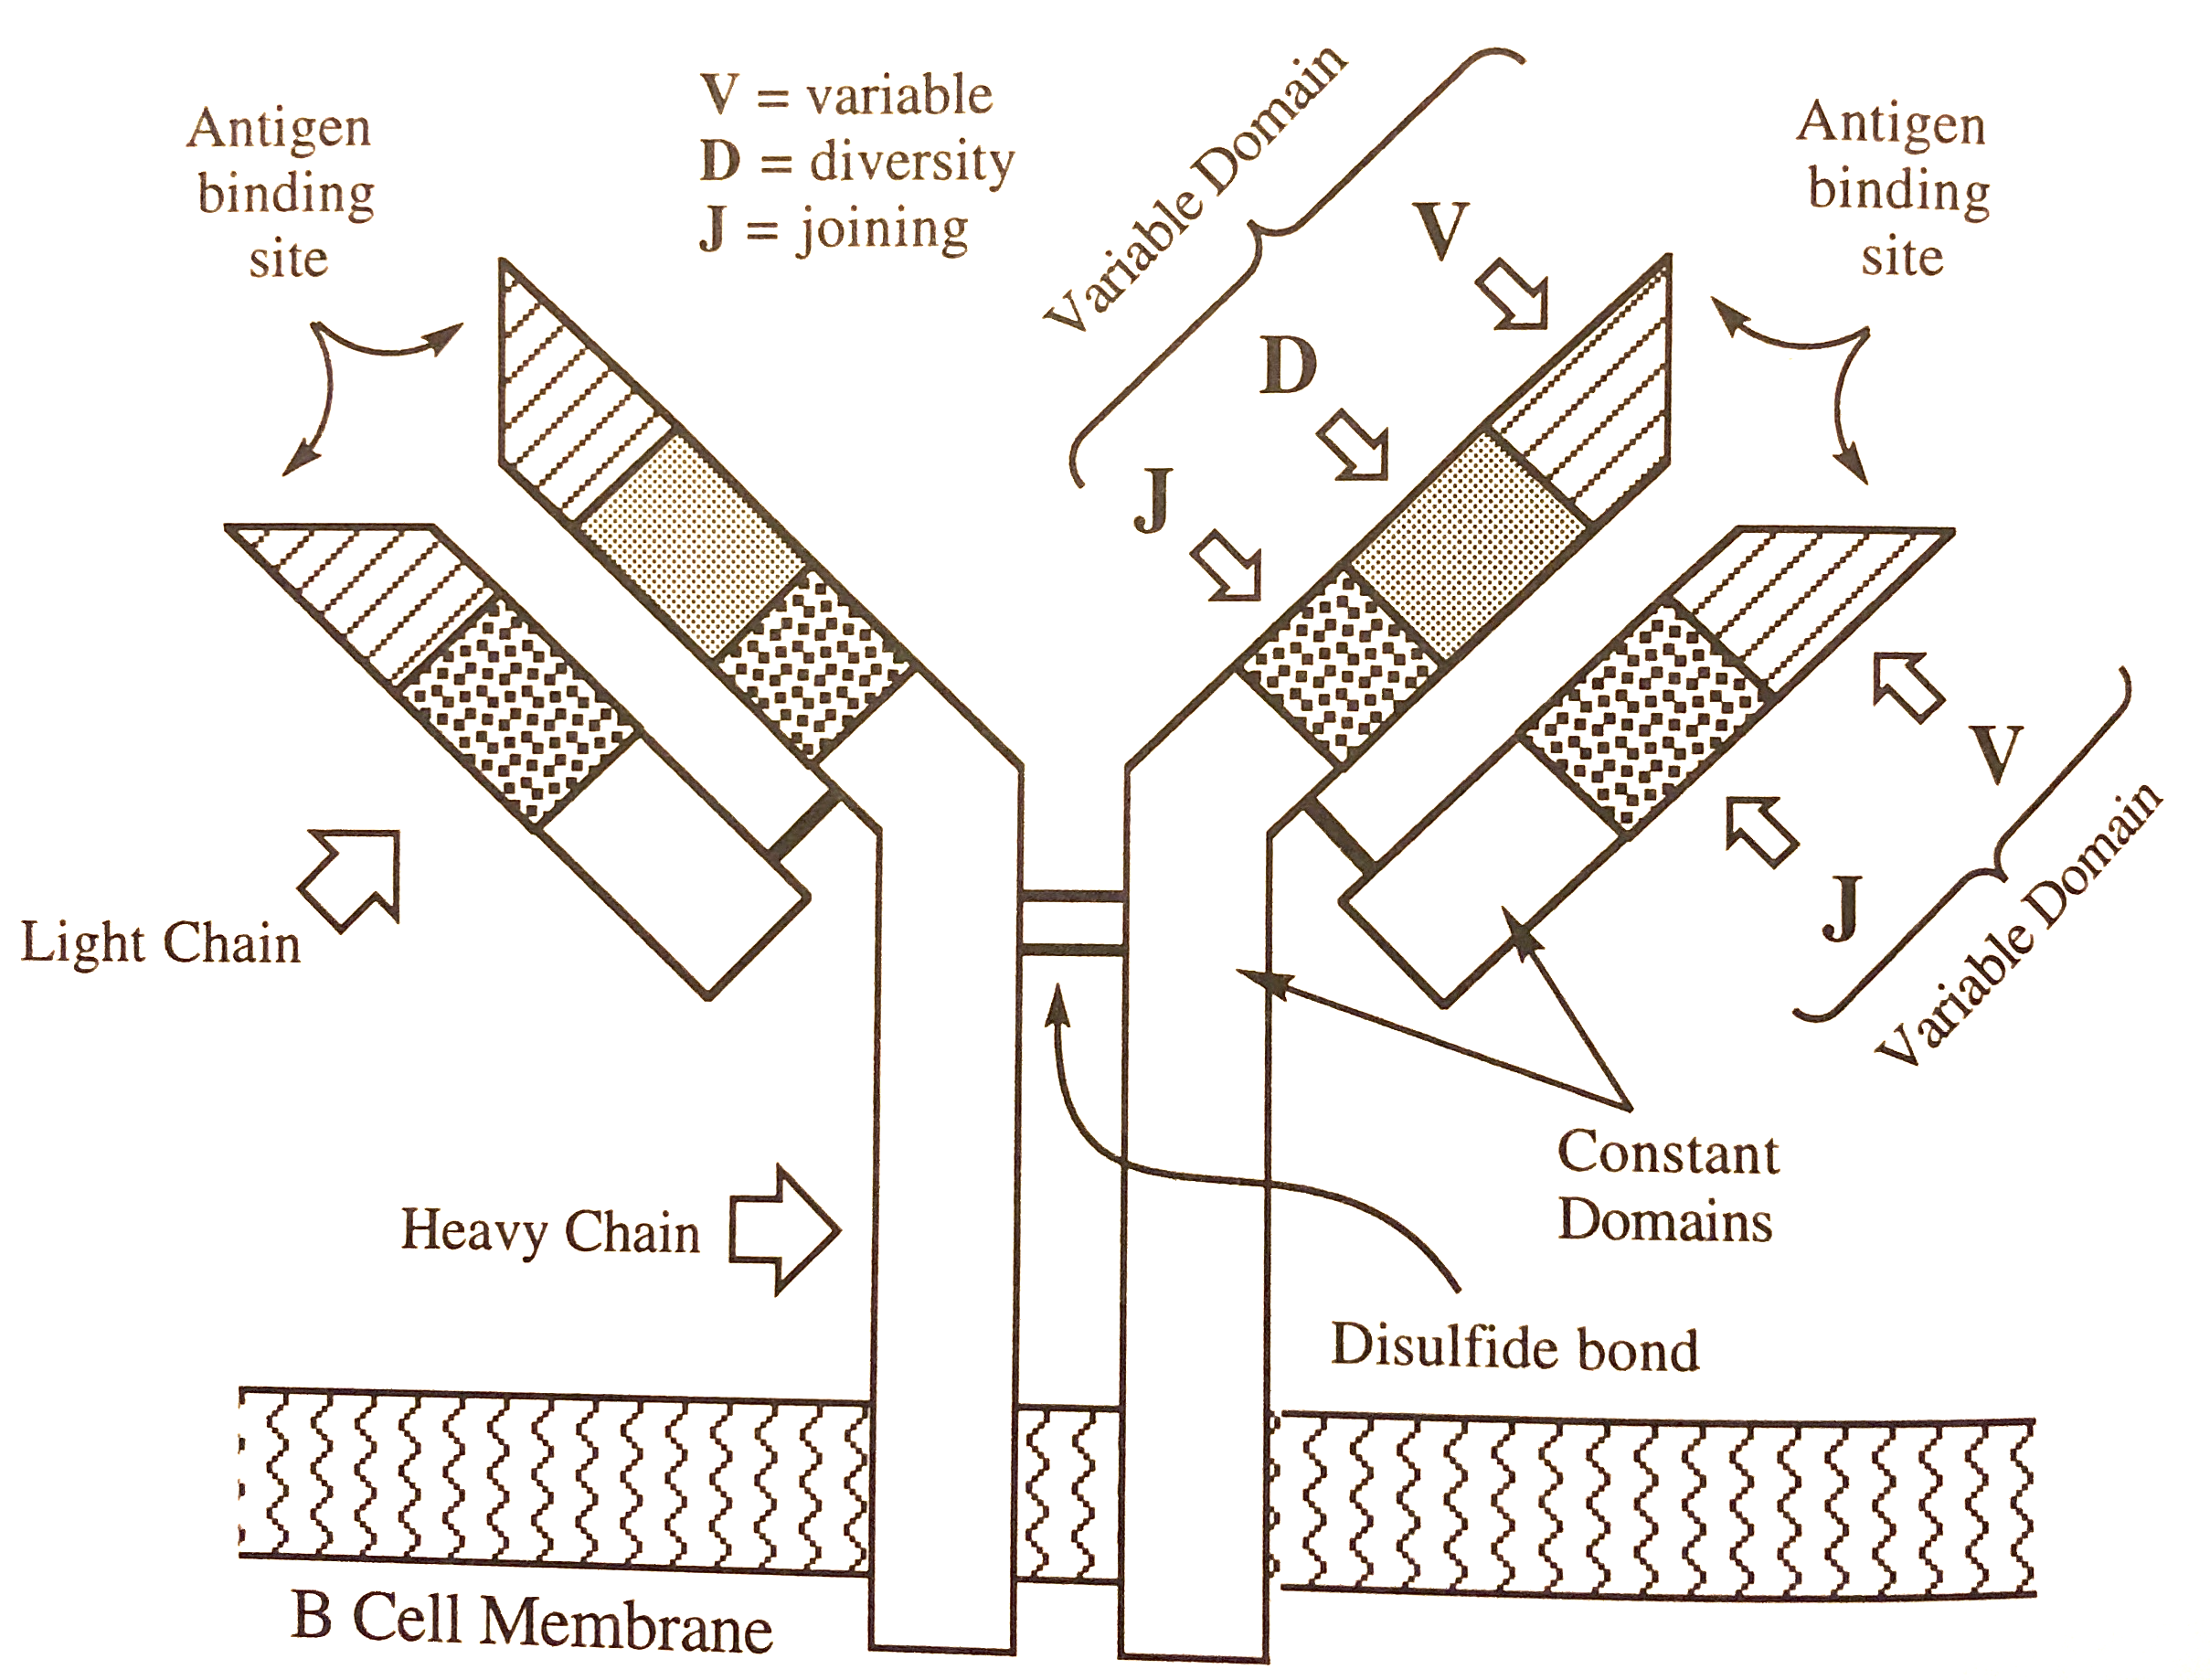
\includegraphics[width=0.7\textwidth]{antibody_structure.png} \label{antibody_structure}
\caption{Example of favorable hydride shift to generate tertiary carbocation from secondary carbocation intermediate.}
\end{figure}
\noindent There are five classes of immunoglobulins that differ in the composition of their heavy chains:
\begin{itemize}
	\item \textbf{IgA:} Found in milk and helps to protect nursing infants.
	\item \textbf{IgD:} Has unknown function.
	\item \textbf{IgE:} Binds to mast cells and is involved in the allergic reaction.
	\item \textbf{IgG:} The only antibody able to cross the placenta. It is also the most abundant and is produced within days after the IgM antibody is secreted.
	\item \textbf{IgM:} Produced a few days after detection of an antigen and it is the first antibody produced in response to an antigen.
\end{itemize}
\noindent Antibodies simply recognize and identify foreign antigens, and can have different mechanisms by which to accomplish this function:
\begin{itemize}
	\item \textbf{Direct Blocking:} The antibody directly blocks the foreign invader from gaining access to host cells. This is accomplished by the antibodies binding to the antigens or other parts of the pathogen.
	\item \textbf{Complement:} An antibody has already recognized and bound to a specific antigen on a bacterial cell that is considered an intruder, and a complement protein (plasma protein) this antigen-antibody complex and binds to the Fc domain of the antibody. After a series of reactions, the complement protein is activated and triggers an immune response. Further reactions form a \textbf{membrane attack complex (MAC)} that inserts into the bacterial cell's membrane and forms a channel that lets water into the cell, causing it to swell with water and eventually lyse.
	\item \textbf{Coating the Cell Surface:} Antibodies can bind to specific antigens on the surface of a bacterial cell and coat the cell surface. Once the antibodies have attached to the bacterial cell, phagocytes and/or killer T cells can bind to the terminal portion of the Fc domain of the antibodies and begin to engulf the foreign invader.
\end{itemize}

\subsection{T Cells}
The receptors for T cells are composed of two polypeptide chains, each with a constant and variable domain. Within a variable domain in each polypeptide we find a variable (V) region and a joining (J) region. On one of the polypeptide chains is a diversity (D) region. 
\begin{figure}[h!]
\centering
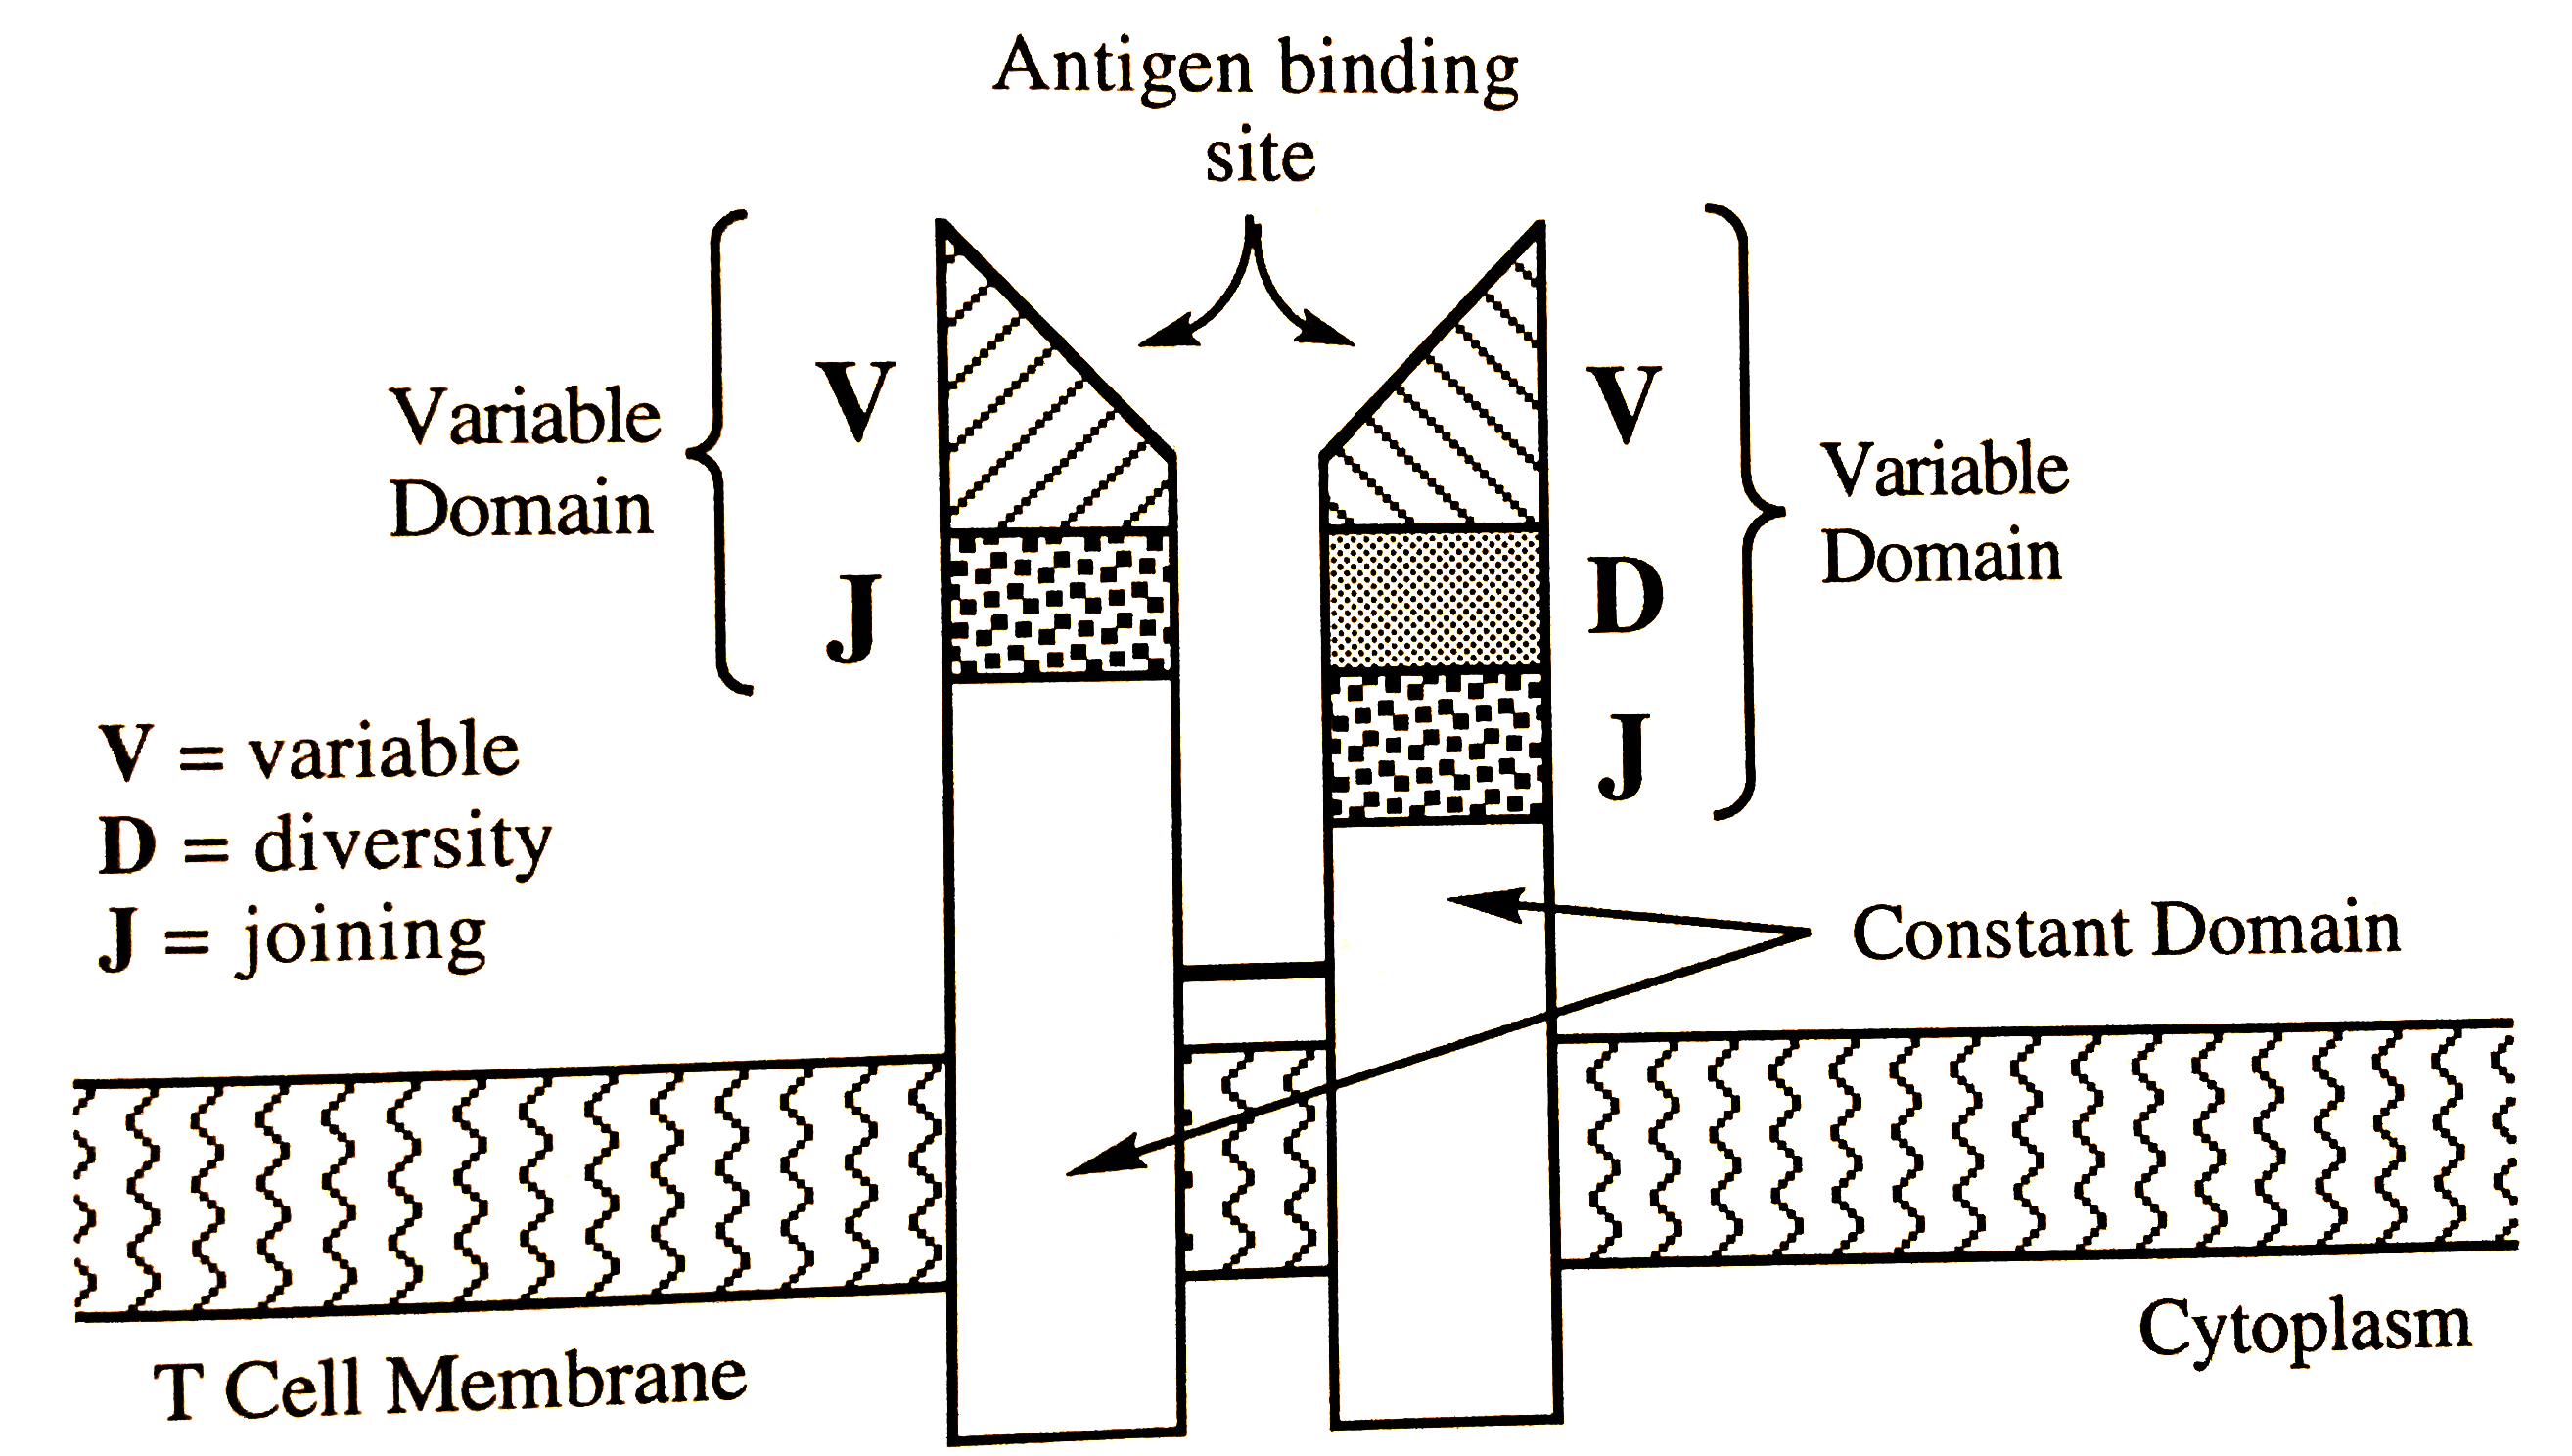
\includegraphics[width=0.55\textwidth]{t_cell_receptor.png} 
\caption{Example of T-cell Receptor Structure}
\end{figure}
\noindent If a virus infects a host cell, then that virus will begin to take over the host's metabolic machinery. As this happens some of the viral antigens are transported to the surface of the host cell where they can complex with a MHCI protein receptor, which are found on almost every one of our cells. The antigen-MHCI complex is recognized by the cytotoxic T cells, which induce lysis in the host cell. Immature helper T cells recognize macrophages which have presented an antigen on their MHCII receptors. Binding induces the macrophage to synthesize and release IL-1, which acts on the immature helper T cell and causes it to release IL-2, further stimulating the immature helper T cell to proliferate into a mature helper T cell. The mature form of the helper T cell secretes IL-2 which can activate cytotoxic T cells, B cells, and more helper T cells. 

\subsection{Immunology\textemdash Generalized Review}
Let's summarize the basic events in humoral and cellular immunity:
\begin{enumerate}
	\item A virus/bacterium enters the body by the blood and is engulfed by a macrophage.
	\item On the surface of the macrophage are MHCI receptors and MHCII receptors.
	\item A MHCII receptor presents the viral antigen to the receptor of a helper T cell, causing the macrophage to release IL-1 that stimulates the helper T cell to proliferate. 
	\item The helper T cell is stimulated to release IL-2 which enhances proliferation of helper T cells.
	\item A B cell with a MHCII protein presents viral antigen to helper T cells, and the IL-2 released from helper T cells stimulates B cells to proliferate.
	\item B cells produce plasma cells and memory B cells. Memory B cells `remember' antigen and proliferate faster during a future invasion of the same virus. Plasma cells secrete antibodies specific for the viral antigen. 
	\item The antibodies respond by direct block, complement, and cell surface coating.
	\item IL-2 from the helper T cells stimulates cytotoxic T cells which have bound to the MHCI protein-antigen complex of an infected cell to lyse the infected cell.
	\item Interferon is secreted by the infected host cell and acts on the cytotoxic T cell to help enhance the immune response.
	\item Cytotoxic T cell also make memory T cells, which will proliferate faster during a future invasion fo the same virus.
\end{enumerate}
\textbf{Fig. \ref{immune_pathway}} shows a diagram that basically summarizes the above information:
\begin{figure}[h!]
\centering
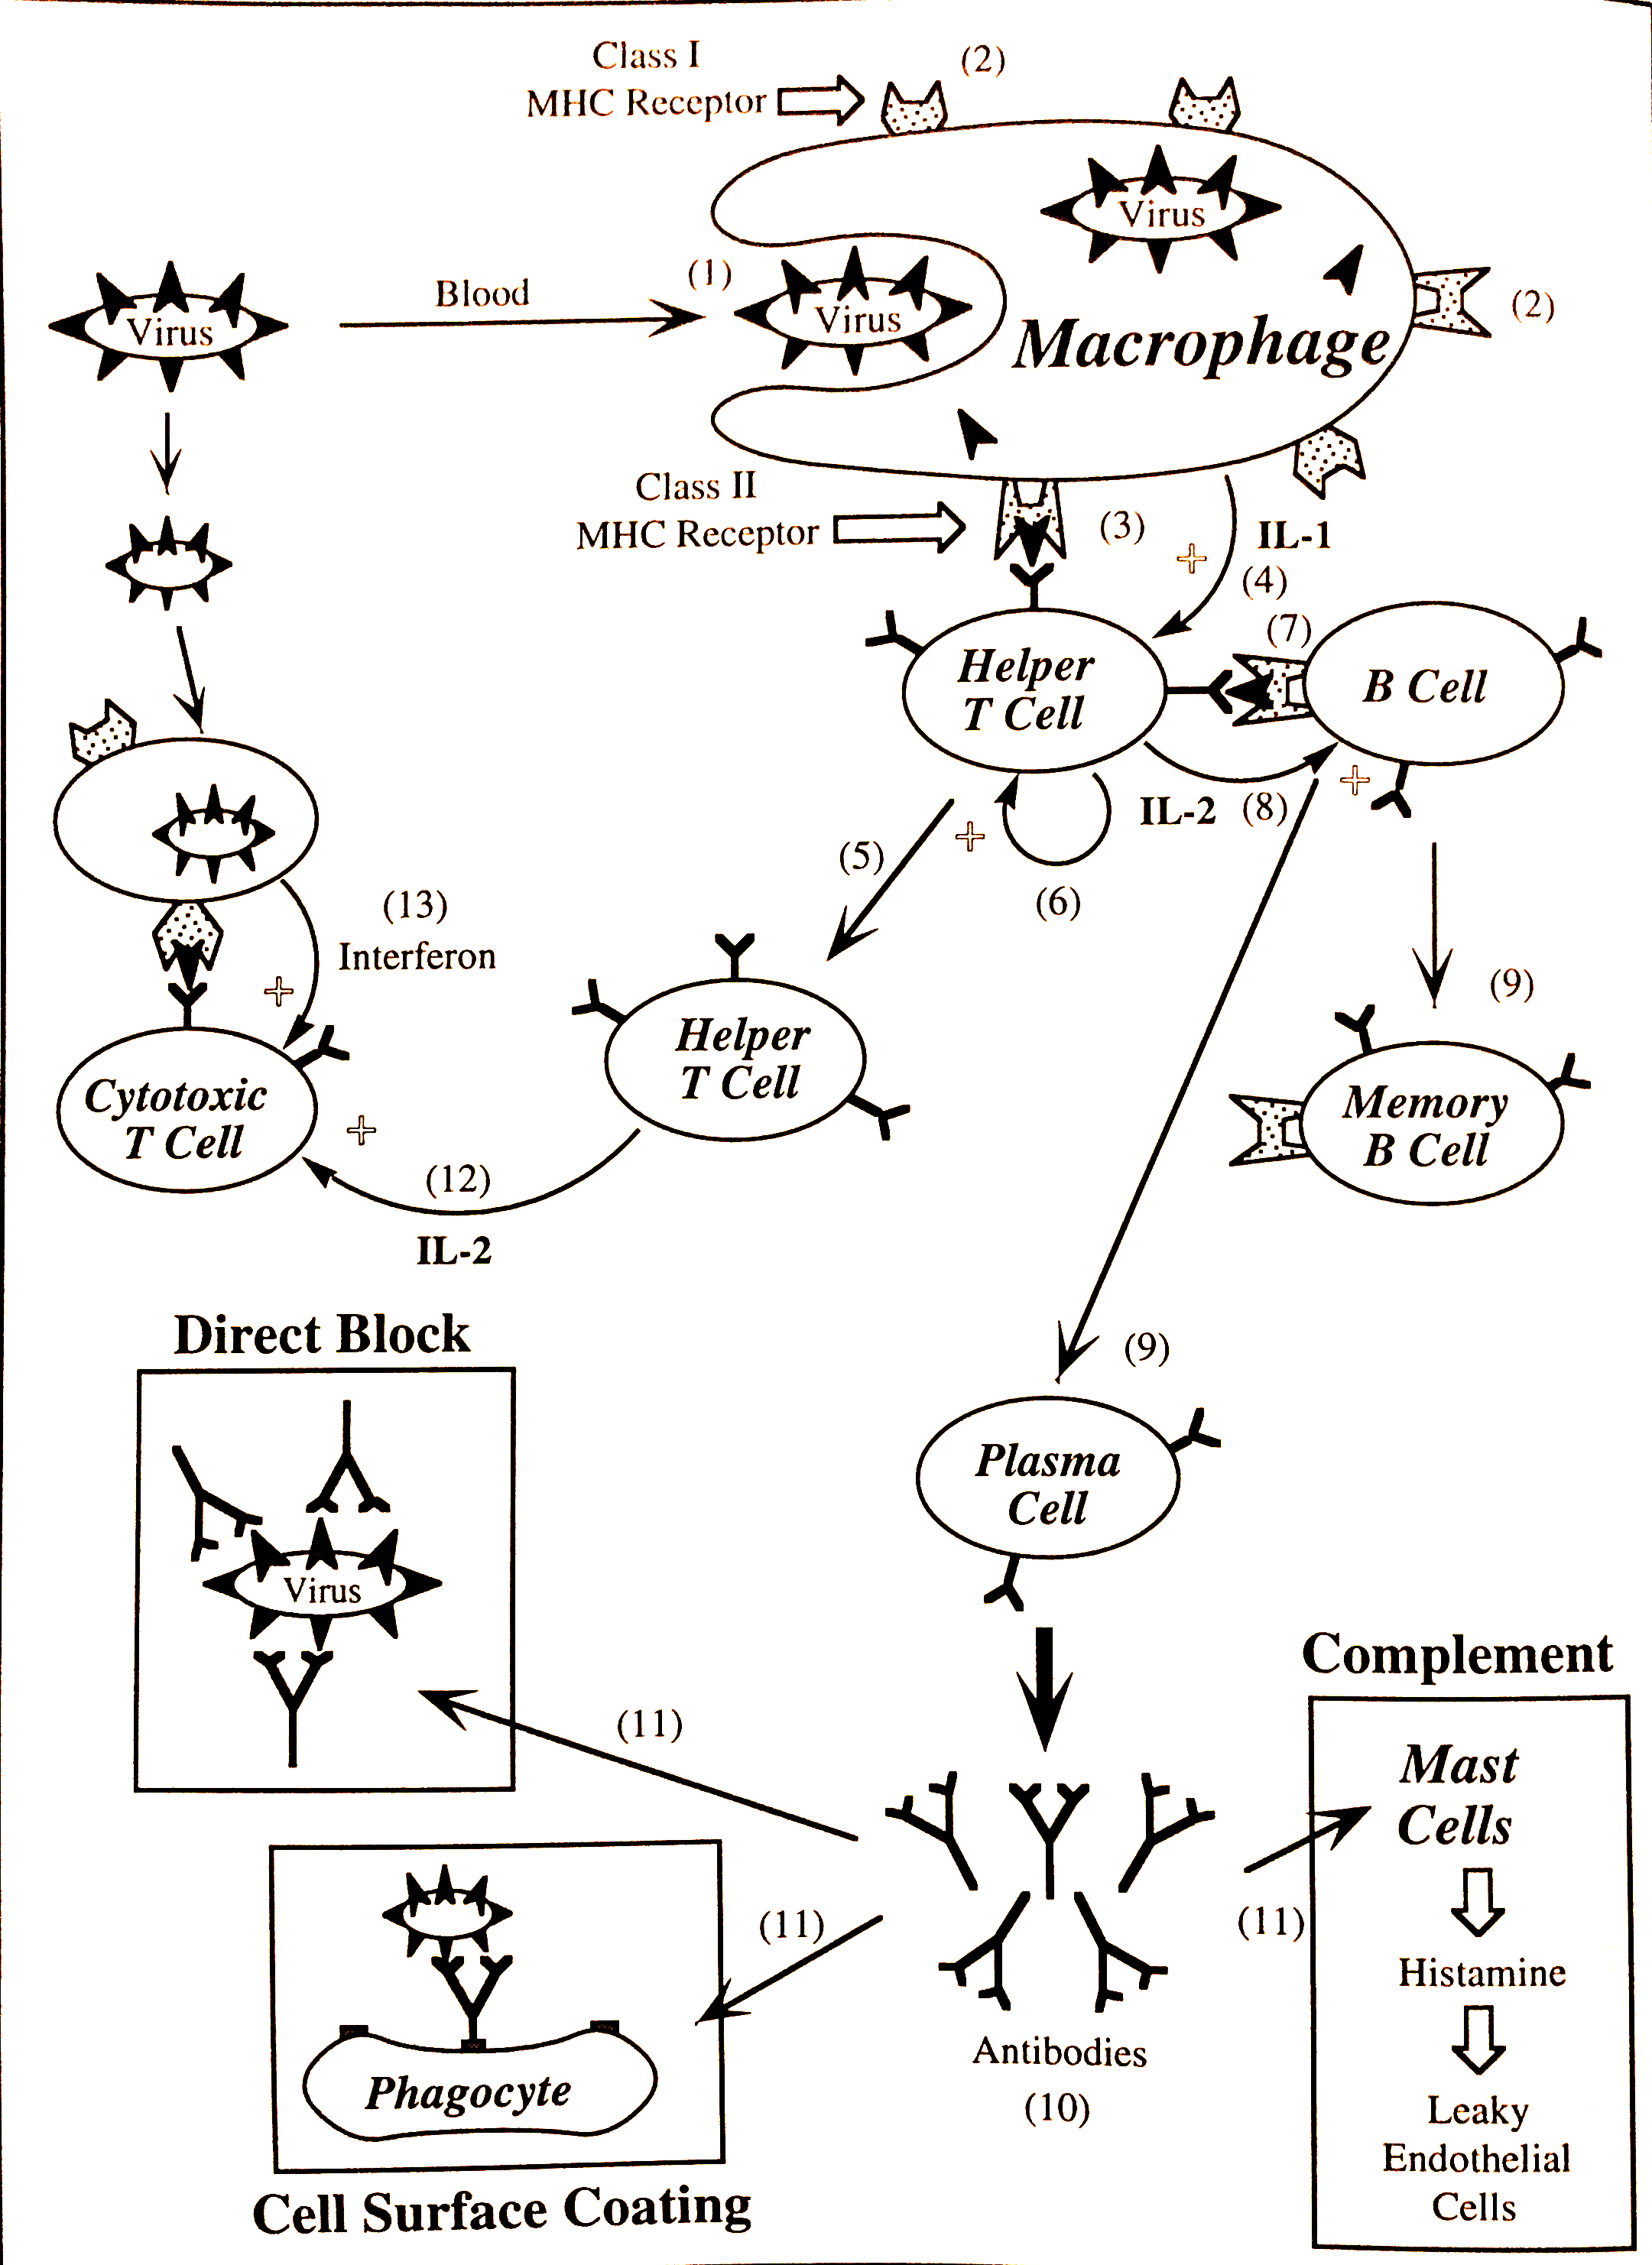
\includegraphics[width=0.7\textwidth]{immune_pathway.png} \label{immune_pathway}
\caption{Review of humoral and cellular immunity pathways.}
\end{figure}

\section{General Chemistry}
\subsection{Stoichiometry}
The MCAT does involve some math, but often it isn't too complicated. Math-related calculations required for MCAT questions involve making approximations, determining ratios, setting up calculations, and estimating the effect of errors on results. Unit conversions to memorize:
\begin{itemize}
	\item Distances: 1 m = 1.094 yd, 2.54 cm = 1 in, 1.609 km = 1 mi
	\item Masses: 1 kg = 2.205 lb, 453.6 g = 1 lb
	\item Volumes: 3.79 L = 1 gal, 1 L = 1.06 qt
	\item Temperatures: $T_F=\frac{9}{5}T_C+32, T_C=\frac{5}{9}\left(T_F-32\right)$
\end{itemize}
\indent \textbf{Molality (m)} is the concentration of a fluid solution defined as the moles of solute per kilogram of solvent. The molality of a solution does not change with temperature, so it is used to calculate the boiling-point elevation and freezing-point depression of solutions containing non-volatile impurities. \textbf{Mass percent} is the concentration of a fluid solution defined as the mass of the solute per mass of solution.\\
\indent Beer's Law is defined to be $\text{Absorbance} = \varepsilon Cl$, where $\varepsilon$ is a constant for the solute at $\lambda_{\text{max}}$ (the wavelength of greatest absorbance), $C$ is the solute concentration, and $l$ is the width of the cuvette. \\
\indent Here are some important solubility rules to remember:
\begin{enumerate}
	\item Most salts containing alkali metal cations (\ce{Li^+}, \ce{Na^+}, \ce{K^+}, \ce{Cs^+}, \ce{Rb^+}) and ammonium (\ce{NH_4^+}) are water-soluble.
	\item Most nitrate (\ce{NO_3^-}) salts are water-soluble.
	\item Most salts containing halide anions (\ce{Cl^-}, \ce{Br^-}, \ce{I^-}) are water-soluble (with heavy metal exceptions such as \ce{Ag^+} and \ce{Pb^2+}).
	\item Most salts containing sulfate anions (\ce{SO_4^{2-}}) are water-soluble (with exceptions such as \ce{Ba^2+}, \ce{Pb^2+}, \ce{Hg^2+}, and \ce{Ca^2+}). 
	\item Most hydroxide anion (\ce{OH^-}) salts are only \textit{slightly} water-soluble. \ce{KOH} and \ce{NaOH} are substantially soluble, while \ce{Ca(OH)_2}, \ce{Sr(OH)_2}, and \ce{Ba(OH)_2} are fairly soluble in water.
	\item Most carbonate anion (\ce{CO_3^{2-}}), chromate anion (\ce{CrO_4^{2-}}), phosphate anion (\ce{PO_2^{3-}}), and sulfid anion (\ce{S^2-}) salts are only slightly water-soluble.
\end{enumerate}
\indent Theres also some general test-taking tips and general advice that could prove very worthwhile:
\begin{enumerate}
	\item Keep in mind that on a multiple-choice exam, the math has been done for you, so all you need to do is approximate the answer.
	\item Intuition will prove useful on the MCAT. As you study for your MCAT, you need to learn to trust your intuition.
	\item Keep in mind that you are \textit{not} graded for showing your work on the MCAT, so don't solve every problem to the last decimal place. Analyze each question only well enough to eliminate three wrong answers. Be concise and efficient in your problem solving, not exhaustive.
\end{enumerate}

\subsection{Atomic Theory}
\hilight{TODO} %TODO

\subsection{Periodic Trends}
The \textbf{effective nuclear charge} $Z_{eff}$ is the net charge exerted upon the valence electrons, which takes into account the shielding from the core electrons. As you move from left to right across a period in the periodic table, the effective nuclear charge increases. Also, as you descend a family/group in the periodic table, the valence shell increases, so the distance between the atom's valence electrons and its nucleus increases. Periodic trends depend on both $Z_{eff}$ and the valence shell. As you move up the periodic table and to the right, the following general atomic trends are observed:
\begin{enumerate}
	\item The atomic size decreases (the radius of the atom is defined as the distance from the center of the nucleus to the exterior of the valence electron cloud).
	\item The ionization energy increases (the energy required to remove the outermost electron from the atom in its gas phase).
	\item The electron affinity increases (the energetics associated with an atom gaining an electron in its gas phase).
	\item The electronegativity increases (the tendency to hold shared electrons with another atom within a bond). 
\end{enumerate}
\noindent Note that each trend shows some deviation from uniformity, some more than others. The effective nuclear charge does not uniformly increase when we scan left-to-right across a period. Half-filled stability and filled-shell stability cause some of the common deviations seen with electron affinity and ionization energy. For instance, nitrogen has a larger ionization energy than oxygen, because upon ionization, nitrogen loses its half-filled $p$-shell. On the contrary, oxygen gains half-filled stability upon being ionized.\\
\indent As a general rule, cations are smaller than neutral atoms because the loss of electrons allows the atom to compact more tightly. As a general rule, anions are larger than neutral atoms, because the gain of electrons causes the atom to expand given the enhanced repulsion associated with the additional electrons.\\
\indent Helium has a larger \textbf{atomic radius} than hydrogen. This is because the electrons in the $n=1$ level repel one another more than the electrons in any higher quantum level because they have the smallest interelectronic distance. This repulsion forces the electrons away from one another in helium, resulting in a greater area begin occupied by the orbiting electrons, and hence a greater radius for helium. \\
\indent \textbf{Ionization energy} is the energy required to remove a valence electron when the element is in the gas phase. The generic ionization reaction is represented by the equation \ce{E(g) -> E+(g) + e-}, where \ce{E} represents any element. Notable exceptions to the general ionization energy trend occur when there is half-filled stability of the energy level and where there is an $s^2$-shell. In both cases, the ionization energy is higher than expected, and also higher than the ionization energy of adjacent elements in terms of atomic number in most cases we'll be considering. \\
\indent \textbf{Electron affinity} measures the tendency of an element to gain an electron; it can be either negative or positive, meaning that gaining an electron to the valence shell can be either exothermic or endothermic. The generic reaction is represented by the equation \ce{E(g) + e- -> E-(g)}, where \ce{E} represents any element. The biggest deviations are attributed to the stability associated with a filled $s$-shell. For instance, the sudden increase in electron affinity from \ce{Be} to \ce{B}, \ce{Mg} to \ce{Al}, and \ce{Ca} to \ce{Ga} is attributed to the instability of one electron in the $p$-level. No trend for electron affinity is evident in the transition metals. \\
\indent \textbf{Electronegativity} is the ability of an atom to attract towards itself the electrons within a chemical bond. The trend in electronegativity is pretty clean, showing no exceptions at least in the first 20 elements.

\subsection{Important Periodic Families}
All alkali metals are strong reducing agents and react favorably with water in the reaction \ce{2M(s) + 2H_2O(g) -> 2MOH(aq) + H_2(g)}. The oxides they form are variable with the metal. Lithium forms \ce{Li_2O}, sodium forms a peroxide \ce{Na_2O_2}, and potassium, rubidium, and cesium form superoxides \ce{MO_2}. Alkali metals can also be oxidized into cations by halogens, nitrogen, and hydrogen. \\
\indent Alkaline earth metals are not as soluble in water as are the alkali metals in their cation form, primarily due to their \ce{2+} charge and smaller radius. They can react favorably with water (except for Be) according to the reaction \ce{M(s) + 2H_2O(g) -> M(OH)_2(aq) + H_2(g)}. The alkaline earth metals all form oxides \ce{MO} when oxidized by oxygen gas. They can also be oxidized by halogens, nitrogen, and hydrogen.\\
\indent Chalcogens are the sixth group of the periodic table that includes oxygen, sulfur, selenium, tellurium, and polonium. As neutral elements, they are oxidizing agents, but their reactivity decreases as you descend the column. Oxygen exists as a diatomic molecule \ce{O_2}, sulfur and selenium exist as octatomic molecules \ce{S_8} and \ce{Se_8}, and tellurium and polonium exist in vast molecular matrices.\\
\indent Halogens and noble gases are also important but nothing's new here. When exposed to high concentrations of fluorine gas, xenon and krypton are known to form molecular compounds with fluorine. The resulting xenon fluorides and krypton fluorides show more electron density around fluorine than the noble gas, implying that fluorine is more electronegative than either xenon or krypton. Otherwise, noble gases are pretty much unreactive. 

\subsection{Electrochemistry}
\hilight{TODO} %TODO

\subsection{Gases and Gas Laws}
\hilight{TODO} %TODO

\subsection{Phases and Phase Changes}
\hilight{TODO} %TODO

\section{Organic Chemistry of Biological Systems}
\subsection{Molecular Structure}
For nonpolar $\sigma$ bonds, most of the electron density is \textit{between} the nuclei. This means that when drawing electron cloud diagrams, the $\sigma$ bond looks more like an ellipsoid as opposed to a dumbbell.\\
\indent The more substituted a carbon atom is, the less strong bonds it is able to form. This is because the other groups are able to (mildly) take electrons away from the bond of interest and thus make it weaker. Bonds involving $sp^3$ carbons are the weakest, while those involving $sp$ carbons are the strongest, because they have the most $s$ character. And of course, triple bonds are the strongest, while single bonds are the weakest, because of the number of electrons shared between atoms. For example, consider the molecule shown in Figure \ref{oc:1.4}.
\begin{equation}
\begin{split}
\chemfig{
           \mcfatomno{1}% 1
    -[:320]\mcfatomno{2}% 2
              (
        -[:260]\mcfatomno{13}% 13
                  (
            -[:320]\mcfatomno{15}% 15
                  )
        -[:200]\mcfatomno{14}% 14
              )
     =[:20]\mcfatomno{3}% 3
              (
         -[:80]\mcfatomno{5}% 5
              )
    -[:320]\mcfatomno{4}% 4
              (
        <[:260]H\mcfatomno{6}%\mcfright{H}{\mcfatomno{6}}% 6
              )
              (
       <:[:220]\mcfatomno{7}% 7
              )
     -[:10]\mcfatomno{8}% 8
              (
        <:[:60]H\mcfatomno{9}%\mcfright{H}{\mcfatomno{9}}% 9
              )
              (
      -[:287.5]\mcfatomno{11}% 11
              )
     <[:25]\mcfatomno{10}% 10
    -[:325]\mcfatomno{12}% 12
}
\end{split} \label{oc:1.4}
\end{equation}
Here, let us consider Bonds A (1 and 2), B (2 and 3), C (2 and 13), and D (4 and 8). Between these four bonds, B is the strongest since it is a double bond. D is the weakest because it is between two $sp^3$-hybridized carbons. Bond A is stronger than bond C, despite both sharing an $sp^2$-hybridized and $sp^3$ hybridized carbon, because bond C contains the more highly substituted carbon.\\
\indent Hybridization of carbon atoms can affect the acidity of hydrogens bound to them. Contrary to most other acids, as the hybrid orbital gets smaller, the electrons are held closer to the nucleus of the atom boned to hydrogen, so the bond can be cleaved in a heterolytic fashion more easily. The more $s$-character in the hybrid orbital of the atom bonded to the hydrogen, the stronger the acid. This results in the relative acidity being $sp>sp^2>sp^3$. This trend is most commonly observed with \ce{C} acidity, but can also be observed with \ce{N} and \ce{O}.\\
\indent Steric hindrance occurs any time two atoms attempt to be in the same place at the same time. It is repulsive in nature and increases as the atoms draw closer. On cyclohexane, substituents with axial orientation experience greater steric hindrance than substituents with equatorial orientation. Thus, substituents (especially the bulky ones) prefer to be in the equatorial position.\\
\indent \textit{Intermolecular forces are the primary consideration} when approximating physical properties (i.e. boiling point). If IMFs are not enough, you also need to consider the molecular mass and molecular rigidity of the molecules. Heavier compounds have higher boiling points, and compounds with greater molecular flexibility can twist and conform to allow for more surface area, and thus more intermolecular interactions. This is why cell membranes would be most rigid if their fatty acids were completely saturated and long molecules, as interactions are greatest with long, saturated fatty acids. \\
\indent The best micelles has an ionic (charged) head and a long carbon chain for the organic tail. For example, \ce{H_3C(CH_2)_{14}CO_2^-} is a better micelle than \ce{H_3C(CH_2)_{14}CO_2H} because it has a charged head, which is more hydrophilic than even the polar, protic carboxylic acid.\\
\indent The inductive effect can be applied to both electron withdrawal (i.e. with the canonical example of nearby halogens) and electron donation. For instance, methyl amine is more nucleophilic than ammonia (\ce{NH_3}) because the methyl group is electron-donating. Varying the $R$-group changes the inductive effect. It also changes the size of the molecule, so steric hindrance can affect the reaction. For instance, \ce{(H_3C)_3N} is less nucleophilic than \ce{(H_3C)_2NH} because the electron donation by the additional methyl group does not compensate for the increase in molecular size.\\
\indent Stereochemistry prefixes, to denote orientation:
\begin{itemize}
\item \textbf{R vs. S} R is clockwise around a stereocenter, S is counterclockwise. This convention is used for chiral centers.
\item \textbf{E vs. Z} E is high priority groups on opposite sides of the double bond. Z is high priority groups are on the same side of the double bond. This convention is used for double bonds.
\item \textbf{$\alpha$ vs $\beta$} $\alpha$ means that the hydroxyl group attached to \ce{C_1} (atom 8 in Figure \ref{oc:2} for both molecules) and the \ce{-CH_2OH} group at \ce{C_5} (the groups on atoms 2 and 10 in Figure \ref{oc:2} for both molecules) lies on opposite sides of the ring's plane (a \textit{trans} arrangement), while $\beta$ means that they are on the same side of the plane (a \textit{cis} arrangement). This convention is used when discussing the glycosidic bond between sugar molecules. 
\end{itemize}
\begin{equation}
\begin{split}
\chemfig{
            \mcfatomno{15}O% 15
    >:[:330]\mcfatomno{14}% 14
      -[:30]\mcfatomno{13}% 13
               (
          <[:90]O\mcfatomno{16}% 16
               )
     -[:330]\mcfatomno{12}% 12
               (
         <:[:30]O\mcfatomno{17}% 17
               )
     -[:270]O\mcfatomno{11}% 11
     -[:210]\mcfatomno{10}% 10
               (
        <:[:270]\mcfatomno{18}% 18
         -[:330]O\mcfatomno{19}% 19
               )
     -[:150]\mcfatomno{9}% 9
               (
          -[:90]\phantom{14}% -> 14
               )
     <[:210]O\mcfatomno{8}% 8
     >[:150]\mcfatomno{6}% 6
     -[:210]\mcfatomno{5}% 5
               (
        <:[:270]O\mcfatomno{20}% 20
               )
     -[:150]\mcfatomno{4}% 4
               (
         <[:210]\mcfatomno{21}O% 21
               )
      -[:90]\mcfatomno{3}% 3
               (
         <[:150]\mcfatomno{22}O% 22
               )
      -[:30]\mcfatomno{2}% 2
               (
         -[:330]O\mcfatomno{7}% 7
         -[:270]\phantom{6}% -> 6
               )
      <[:90]\mcfatomno{1}% 1
      -[:30]O\mcfatomno{23}% 23
} %lactose 
\quad
\chemfig{
            \mcfatomno{15}O% 15
    >:[:330]\mcfatomno{14}% 14
      -[:30]\mcfatomno{13}% 13
               (
          <[:90]O\mcfatomno{16}% 16
               )
     -[:330]\mcfatomno{12}% 12
               (
         <:[:30]O\mcfatomno{17}% 17
               )
     -[:270]O\mcfatomno{11}% 11
     -[:210]\mcfatomno{10}% 10
               (
        <:[:270]\mcfatomno{18}% 18
         -[:330]O\mcfatomno{19}% 19
               )
     -[:150]\mcfatomno{9}% 9
               (
          -[:90]\phantom{14}% -> 14
               )
     <[:210]O\mcfatomno{8}% 8
    >:[:150]\mcfatomno{6}% 6
     -[:210]\mcfatomno{5}% 5
               (
        <:[:270]O\mcfatomno{20}% 20
               )
     -[:150]\mcfatomno{4}% 4
               (
         <[:210]\mcfatomno{21}O% 21
               )
      -[:90]\mcfatomno{3}% 3
               (
        <:[:150]\mcfatomno{22}O% 22
               )
      -[:30]\mcfatomno{2}% 2
               (
         -[:330]O\mcfatomno{7}% 7
         -[:270]\phantom{6}% -> 6
               )
      <[:90]\mcfatomno{1}% 1
      -[:30]O\mcfatomno{23}% 23
} %maltose
\label{oc:2}
\end{split}
\end{equation}
\noindent The molecule on the left is lactose with a $\beta$ glycosidic bond, while the molecule on the right is maltose with an $\alpha$ glycosidic bond.\\
\indent The nitrogen atom in amides have planar geometry even if it doesn't appear like it! This is because of the resonance with the carbonyl oxygen group, as shown here:
\begin{equation}
\begin{split}
\begin{bmatrix}
\chemfig{
           O\mcfatomno{1}% 1
    =[:270]\mcfatomno{2}% 2
              (
        -[:330]{NH_2}\mcfatomno{3}% 3
              )
    -[:210]\mcfatomno{4}H% 4
}
\quad\begin{matrix}
\\
\\
\text{\ce{<=>}}
\end{matrix}\quad
\chemfig{
           {O^-}\mcfatomno{1}% 1
    -[:270]\mcfatomno{2}% 2
              (
        =[:330]{NH_2^+}\mcfatomno{3}% 3
              )
    -[:210]\mcfatomno{4}H% 4
}
\end{bmatrix}
\end{split}
\end{equation}
\noindent In this case, we can see that due to resonance, all of the atoms are coplanar for the amide. Quite separately, consider the following example problem:
\begin{center}
\begin{minipage}{30em}
\textcolor{blue}{20. \quad The STRONGEST hydrogen bond is formed between:
\begin{enumerate}[label=\Alph*]
	\item the lone pair of O and a hydrogen bonded to O.
	\item the lone pair of N and a hydrogen bonded to O.
	\item the lone pair of O and a hydrogen bonded to N.
	\item the lone pair of N and a hydrogen bonded to N.
\end{enumerate}}
\end{minipage}
\end{center}
\noindent The answer to this question is answer choice B. This is because the strongest hydrogen bond is formed when the hydrogen is extremely electron deficient (i.e. through being bonded to an oxygen) and it is hydrogen-bonded to something that is extremely basic (or in other words, is very good at donating its electrons in order to create the bond, which best describes the lone pair on a nitrogen atom). \\
\noindent \footnotesize \textit{End of Sunday, June 16, 2019.}
\normalsize

\subsection{Isomers and Stereochemistry}
Isomers can be constitutional/structural (meaning they differ in connectivity of bonds) or stereoisomers (meaning they differ in the spatial arrangement of the atoms). Stereoisomers can either be conformers or configurational isomers. Conformers can differ by orientation in space, and are identical after a specific rotation about a $\sigma$-bond. Configurational isomers also differ by orientation in space, but you can't rotate them to become identical. Configurational isomers can be categorized as either enantiomers or diastereomers. \textbf{Enantiomers} are nonsuperimposable mirror images, while \textbf{diastereomers} are nonsuperimposable structures that are not mirror images. Configurational isomers can also be categorized as either optical isomers or geometrical isomers. \textbf{Optical isomers} rotate plane-polarized light and cannot be rotated to become identical due to the asymmetry in the structure, while \textbf{geometrical isomers} are structures with limited rotation, and can't be rotated to become identical due to the presence of a ring or $\pi$-bond. Geometrical isomers are sometimes also called \textit{cis/trans} isomers. The two categorizations are not mutually exclusive. \\
\indent The Chan-Ingold-Prelog Rules are used to determine the \textbf{absolute configuration} ($R$ vs. $S$) for a stereocenter. The rules are as follows:
\begin{enumerate}
	\item First, you must prioritize the substituents that are attached to the carbon of the stereocenter according to the atomic mass of the atom directly bonded to the chiral carbon (from heaviest atom to lightest atom).
	\item Next, orient the molecule in such a way that the substitutent with the lowest priority points behind the plane of the molecule.
	\item Finally, draw a semicircular arc from substituent 1 through substituent 2 and on to substituent 3. If the arc is clockwise, then the stereocenter is referred to as $R$. If the arc is counterclockwise, then the stereocenter is referred to as $S$. 
\end{enumerate}
\noindent Optical rotation is a characteristic feature of enantiomers that are described by absolute configurations. If, say, the $R$-enantiomer of a compound rotates the light in a positive direction (meaning clockwise) by $X$ degrees, then the $S$-enantiomer of the compound rotates light by $X$ degrees in the negative direction. However, in actuality, the $R$-enantiomer doesn't always rotate light in the positive direction\textemdash it really depends on the identity of the compound of interest.\\
\indent For compounds with multiple chiral centers, here is another way of thinking about enantiomers vs. diastereomers:
\begin{enumerate}
	\item \textbf{Enantiomers} are configurational isomers in which \textit{all} of the chiral centers in each molecule are different from one another.
	\item \textbf{Diastereomers} are configurational isomers in which \textit{at least one, but not all} of the chiral centers in each molecule is different from one another. 
\end{enumerate}
\indent For \textit{geometrical isomers}, which have different spatial arrangements about a $\pi$-bond, the prefix of E is given for trans orientation of the two highest priority groups, while Z is given for cis orientation of the two highest priority groups. \\
\indent \textbf{Meso compounds} are individual structures which contain a mirror plane slicing through the middle of the compound and an \textit{even number} of chiral centers symmetrically displaced about the mirror plane. The net optical rotation of a meso compound is 0 degrees because the opposing chiral centers on each half of the molecule cancel one another out, leaving no net rotation of plane polarized light. A meso compound may be identified by either an inversion center in the middle of the molecule, or a mirror plane through the middle of the molecule.\\
\indent When a molecule contains more than one chiral center, the maximum number of stereoisomers increases exponentially with each new chiral center according to the equation
\begin{equation}
\begin{split}
\text{Number of stereoisomers}=2^n
\end{split}
\end{equation}
\noindent where $n$ is the number of chiral carbons in the molecule. There are less than $2^n$ stereoisomers if one of the possible structures is meso. If $n$ is odd, however, there can't be a meso compound, meaning that there must be exactly $2^n$ stereoisomers.\\
\indent Rotational about $\sigma$ bonds allows for different conformers. The two extreme overall structures are known as \textit{staggered} (where substituents on the first atom do not block the substituents on the back atom of the $\sigma$ bond in question) and \textit{eclipsed} (where substituents on the first atom do block the substituents on the back atom of the $\sigma$ bond in question). Within staggered conformation, the terms \textit{gauche} and \textit{anti} describe the relative position of substituents on adjacent atoms. \textit{Gauche} conformers have the two groups of interest (often the largest groups) having a dihedral angel of 60 degrees, while \textit{anti} conformers have the two groups of interest having a dihedral angle of 180 degrees. Staggered and anti is the most stable, because steric repulsion is minimized. To understand these different types of conformers, take a look at the Newman projections shown in Figure \ref{conformers}.\\
\hilight{Insert Newman projection figures here}. \\
Cycloalkanes are basically cyclic alkanes that have one ring with the chemical formula \ce{C_nH_{2n}} and contain no $\pi$-bonds. Three- and four- membered rings are reactive, while five- and six- membered rings are stable. The reactivity of tree- and four- membered rings is attributed to \textit{ring strain}, defined as the energy difference between the linear and cyclic alkanes of equal carbon length. Let's look at a couple of particularly important cycloalkanes:
\begin{itemize}
	\item Cyclopentane does not require much distortion of its bonds and shape to accommodate the $109.5^{\circ}$ angle for the $sp^3$ hybrid. To achieve the correct angle and alleviate the torsional strain, cyclopentane forms an \textit{envelope shape} where one of the carbons is not coplanar with the other four. However, even with this envelope shape, the substituents on the ring that are in an eclipsed conformation as a result of the near-planar ring structure are unfavorable, causing further contortion of the structure, which accounts for the ring strain energy. 
	\item Cyclohexane has the most stable ring structure of all of the cycloalkanes. The most stable form is the \textit{chair} conformation. Cyclohexane can flip between different chair conformations in a process called \textit{ring-flipping}, and the interconversion process requires that it passes through the \textit{boat} conformation. Equatorial positions (in the plane of the molecule) are more stable than axial (above and below the plane of the molecule), so the most stable conformation of a cyclohexane compound has the largest substituents in the equatorial positions.
\end{itemize}
\hilight{Insert equatorial, axial pictures fo cyclohexane, envelop shape for cyclopentane.}\\
\indent \textbf{Separating Stereoisomers:} In organic chemistry, there are compounds known as \textit{chiral auxiliaries}, which introduce chirality to, or exaggerate existing chirality within, a reactant molecule. Chiral auxiliaries serve in a similar fashion to an enzyme. When aiming for one specific stereoisomer, it is easiest to select for it in the reaction. If not, then a mixture of stereoisomers forms and chirally selective separation techniques must be used. Chirally selective separation techniques come in two types: using an enzyme/chirally selective molecule to react specifically with one stereoisomer within the mixture, or invoking chirality in an existing separation technique. As an example for the first technique, if a new functional group is added to only stereoisomer by an enzyme, the two enantiomers now have different physical properties and can easily be separated. Once separated, the same enzyme can be employed to return the compound back to its original form. As an example for the second technique, a column chromatography gel can be made from a pure stereoisomer. If the column is made with an $R$-alcohol for instance, then when a racemic mixture of alcohols is added, the $S$-enantiomer has a greater affinity for the column, and thus has a greater elution time.

\subsection{Nucleophilic Substitution}
The strength of a leaving group can be predicted by the \ce{pK_a} os its conjugate acid. The more stable the leaving group, the less basic the leaving group, and thus the more acidic the conjugate acid of the leaving group. In other words, the strength of a leaving group increases as the \ce{pK_a} of its conjugate acid decreases.\\
\indent A \textit{racemic mixture} is a product mixture that has an even distribution of enantiomers. It is the observed product when the mechanism involves an intermediate where the reactive site is an $sp^2$-hybridized carbon and the molecule is symmetric (i.e. has no other chiral centers). \\
\indent \ce{S_N 2} reactions involve the nucleophile attacking prior to the leaving group leaving in a \textit{backside} attack, essentially pushing the leaving group off of the electrophile. It has a trigonal bipyramidal transition state.
\begin{table}[h!]
\begin{tabular}{p{6.25cm} p{6.5cm} p{5cm}}
\hline
\textbf{Reactant Features} & \textbf{Course of Reaction Features} & \textbf{Product Features} \\
\hline
\hline
The reactivity preference in an \ce{S_N 2} mechanism is $1^{\circ}>2^{\circ}>3^{\circ}$ in terms of electrophiles. & An \ce{S_N 2} mechanism forms a five-ligand transition state during the middle of the reaction. & A single enantiomeric product is formed (i.e. no racemic mixture). \\
An \ce{S_N 2} mechanism is favored with a good nucleophile. & The 5-ligand transition state is the highest energy state and it exists for just a split second. It \textit{cannot} be isolated. & \ce{S_N 2} reactions exhibit second order kinetics. \\
An \ce{S_N 2} mechanism is favored in polar, aprotic solvents such as ethers and ketones. & Steric forces destabilize the transition state by forcing bond angles to values less than $109.5^{\circ}$. & \ce{S_N 2} reactions are one-step reactions, so they have fast rates of formation.\\
\hline
\end{tabular}
\end{table}
\indent \ce{S_N 1} reactions involve the leaving group leaving before the nucleophile attacks. The carbocation intermediate has a long enough lifetime to be detected using spectroscopy. Both rearrangement (e.g. hydride shifts and alkyl shifts) and a mixture of stereoisomers (formed from either front-side or back-side attack of the $sp^2$-intermediate) are observed with \ce{S_N 1} reactions. Formation of the carbocation is the rate-limiting step. \\
\begin{table}[h!]
\begin{tabular}{p{6.25cm} p{6.5cm} p{5cm}}
\hline
\textbf{Reactant Features} & \textbf{Course of Reaction Features} & \textbf{Product Features} \\
\hline
\hline
The reactivity preference in an \ce{S_N 1} mechanism is $3^{\circ}>2^{\circ}>1^{\circ}$ in terms of electrophiles. & Steric hindrance pushes the leaving group off of the electrophile. & A racemic mixture forms when the electrophile has chirality. \\
An \ce{S_N 1} mechanism is seen with a poor nucleophile. & The intermediate is a planar, three-ligand carbocation where the carbon has $sp^2$-hybridization. & \ce{S_N 1} reactions exhibit first order kinetics. \\
An \ce{S_N 1} mechanism is favored in protic solvent such as alcohols. & An intermediate is observed in addition to transition states. & \ce{S_N 1} reactions are slow, two-step reactions.\\
\hline
\end{tabular}
\end{table}
\indent The \ce{S_N 1} reaction can be complicated by \textbf{rearrangement} because of the carbocation intermediate formed. If a secondary carbocation (\ce{R_2CH^+}) is formed, it can rearrange to form a more stable tertiary carbocation (\ce{R_2C^+}) when possible. See Figure \ref{1-2-hydride-shift-mechanism} for an example. Furthermore, if the electrophile has a chiral center at a site other than the electrophilic carbon, an \ce{S_N 1} reaction will form both a major and minor product. The major product results from the transition state with least steric hindrance.
\begin{figure}[h!]
\centering
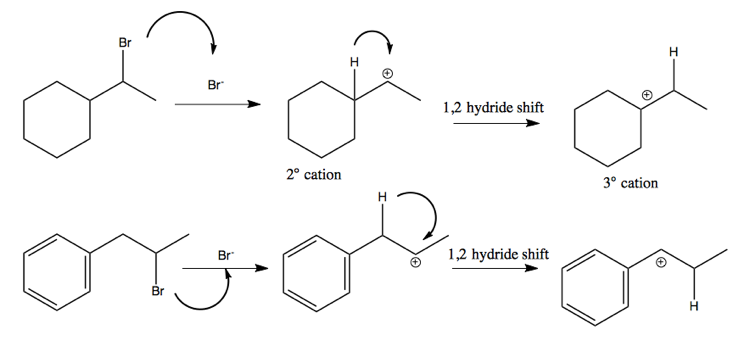
\includegraphics[width=0.7\textwidth]{1-2-hydride-shift-mechanism.png} \label{1-2-hydride-shift-mechanism}
\caption{Example of favorable hydride shift to generate tertiary carbocation from secondary carbocation intermediate.}
\end{figure}
\noindent Primary electrophiles proceed by \ce{S_N 2} while tertiary electrophiles proceed by \ce{S_N 1}. Secondary electrophiles can proceed by either \ce{S_N 1} or \ce{S_N 2}. Also, the stronger the nucleophile, the more likely the reaction will proceed by an \ce{S_N 2} mechanism; the better the leaving group, the more likely the reaction will proceed by an \ce{S_N 1} mechanism. Also, consider the following rate laws:
\begin{equation}
\begin{split}
\ce{S_N 1} \text{ Rate}=k\left[\text{Electrophile}\right]\\
\ce{S_N 2} \text{ Rate}=k\left[\text{Nucleophile}\right]\left[\text{Electrophile}\right]
\end{split}
\end{equation}
\noindent Lastly, you can also consider the solvent to distinguish between \ce{S_N 1} and \ce{S_N 2} reactions: if the solvent is protic (i.e. capable of forming hydrogen bonds), the reaction will have a tendency to proceed by an \ce{S_N 1} mechanism. If the solvent is aprotic (i.e. \textit{not} capable of forming hydrogen bonds), the reaction will have a tendency to proceed by an \ce{S_N 2} mechanism.

\section{Physics}
\subsection{Translational Motion}
In general on the MCAT, although especially for the physics section, it's about speed more than precision. Important kinematic equations that you probably don't know yet:
\begin{equation}
\begin{split}
\Delta x = \frac{1}{2}\left(v_0+v_f\right)\Delta t, \quad v_f^2=v_0^2+2a\Delta x
\end{split}
\end{equation}

\subsection{Forces and Torque}
\indent In order to handle formula identification problems \textit{quickly} (as speed is extremely important on the exam), the two best techniques are \textbf{checking units} and considering \textbf{limiting cases}. For example, consider the following problem:
\begin{center}
\begin{minipage}{30em}
\textcolor{blue}{Example 2.3a\quad The pulley system shown below, sometimes referred to as an \textit{Atwood machine}, has two masses, $m_1$ and $m_2$. Which of the following formulas represents the acceleration of this system?
\begin{enumerate}[label=\Alph*]
	\item $a=\frac{\left(m_1-m_2\right)g}{m_1+m_2}$
	\item $a=\frac{\left(m_1+m_2\right)g}{m_1-m_2}$
	\item $a=\frac{g}{m_1+m_2}$
	\item $a=\frac{m_2g}{m_1+m_2}$
\end{enumerate}}
\end{minipage}
\end{center}
\noindent This problem essentially shows two masses, $m_1$, $m_2$, attached on two sides of the pulley. There's a traditional solution to \textit{actually} solve for the acceleration of the system, shown on pages 57-58 of TBR Physics, but this takes a lot of time. Instead, we can entirely avoid actually `solving' by using the fact that the test is multiple choice. Choices C and D don't have the right units, so they are definitely wrong. Distinguish between A and B by considering limiting cases. If $m_1=m_2$, then it should be zero acceleration, not infinite acceleration, so thus, the right answer is \textbf{A}. See how quickly we were able to arrive at the right answer?!\\
\indent Recall that torque $\mathbf{\tau}$ is defined to be $\mathbf{\tau}=\mathbf{r}\times\mathbf{F}$. The length is sometimes called the \textit{lever arm} or \textit{moment arm}, and the center of the bolt is called the \textit{pivot point}. \\
\indent Although it may sound strange and possibly incorrect when you first consider the idea, it is possible for a static friction to accelerate an object from rest. There are two \textit{everyday} examples that can help you to accept this concept: walking and driving. When you start walking from rest, you are clearly going from $v=0$ to having a velocity in the direction you are moving. This means that you have accelerated. This is achieved by \textit{pushing off} against the ground in a lateral direction. So, there must be a force accelerating you in a lateral direction. According to Newton's third law, there is an equal and opposite force as your push-off force. That opposing force is a static friction of the ground against your foot, as long as your foot does not slip. This explains why it is harder to start walking on an icy floor than a carpeted floow, because the static coefficient of friction $\mu_s$ for ice is much lower than $\mu_s$ for carpet. \\
\indent In physics and engineering, \textbf{mechanical advantage} is the factor by which a machine multiplies the force put into it. The mechanical advantage of a lever/see-saw can be described by the following equation:
\begin{equation}
\begin{split}
\text{mechanical advantage}=\frac{\text{weight of object}}{\text{applied force needed to support object}}=\frac{d_{\text{fulcrum}}}{d_{\text{weight}}}
\end{split}
\end{equation}
\noindent where $d_i$ is the distance from the fulcrum of object $i$. Example problems for force and torque:
\begin{center}
\begin{minipage}{30em}
\textcolor{blue}{9.\quad Which of the following graphs (see Figure \ref{Physics_1_2_9}) best represents the force due to static friction as incline angle increases for a redwood block atop a smooth rubber surface?}
\end{minipage}
\end{center}
\begin{figure}[h!]
\centering
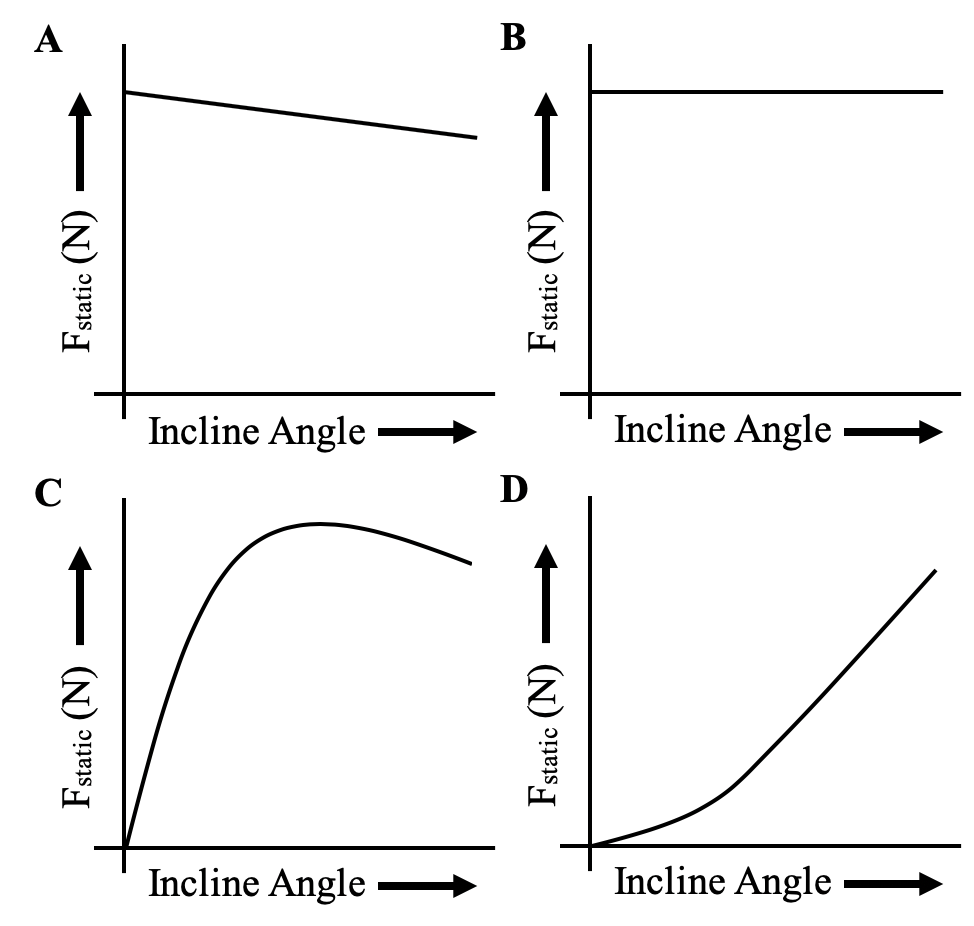
\includegraphics[width=0.4\textwidth]{Physics_1_2_9.png} \label{Physics_1_2_9}
\caption{Answer choices for Question 9 (Taken from Physics Part I, Passage II, Question 9 in TBR)}
\end{figure}
\indent Initially, you'd probably think that the answer is A; as you increase the incline angle, it makes sense the the static friction force would decrease, as this is what happens with the normal force, right? However, recall that static friction is a reactionary force, meaning that it is equal and opposite of any applied force. At zero inclination, the block has no inclination to move or anything like that, so the static friction is 0. As the block has more and more incentive to move as the incline angle increases (due to the force of gravity), the static friction must also increase in order to keep the block in place, until the object breaks free and begins to slide down the surface. Thus, the best answer choice in this instance is \textbf{D}. \\
\begin{center}
\begin{minipage}{30em}
\textcolor{blue}{22. If a person starts at the rim of a spinning platform and is pushed radially toward the central axis by a moving exterior wall, then what happens to the normal force felt by that person due to the wall?
\begin{enumerate}[label=\Alph*]
	\item It remains a constant.
	\item It decreases, since $r$ decreases.
	\item It increases, since $r$ decreases. 
	\item It decreases, since angular speed decreases.
\end{enumerate}}
\end{minipage}
\end{center}
\indent By Newton's third law, we know that the normal force felt by the person is equal to the force the person exerts on the wall, which is basically equal to the centripetal force $F_c=v^2/r$. Superficially, this looks like an inverse relationship $F_c\propto 1/r$, and so we may naively guess the answer is C. However, as $r$ decreases, $v$ also changes for circular motion! Rather, only angular frequency $\omega=v/r$ remains constant, so thus, the form of $F_c$ that we want to use is $F_c=\left(\omega r\right)^2/r=\omega^2r$. From this equation, it is clear that in reality, $F_c\propto r$, and so the correct answer is \textbf{B}.

\subsection{Work and Energy}
When negative work is done \textit{on} an object, it loses energy to its surroundings. Friction takes energy away from the sliding object. Generally, if \textit{positive} work is done \textit{on} the object, the object \textit{gains} energy. If \textit{the object does positive work}, the object \textit{loses} energy. If the work is negative, then the opposite would be true. For example, the work done on a block by friction as it slides on a rough surface is negative and directly proportional to $\mu_k$. The work done on a road surface, as a car skids across it, is positive and directly proportional to the skidding distance. \\
\indent The three forms of energy you need to know are kinetic energy, gravitational potential energy, and spring potential energy. Power is the rate of doing work/transferring energy with respect to time.\\
\indent Two simple machines that occasionally surface on the MCAT are the \textbf{inclined plane} and the \textbf{pulley system}. They make life easier, because they redirect and/or reduce the amount of \textit{force} we need to apply in accomplishing some task. However, they do not lessen the overall amount of work that must be done! It still requires the same amount of energy to carry out the task. This is to say that because energy is conserved, the amount of work needed to perform an action will be constant, no matter how the action occurs. Other simple machines include \textbf{levers} (as we saw in the rotational equilibrium section) and \textbf{hydraulic lifts} (which we will see in the fluids section).\\
\indent One way to characterize a machine is through its \textbf{mechanical advantage}, defined as
\begin{equation}
\begin{split}
\text{mechanical advantage}=\frac{\text{weight of the object to be supported}}{\text{applied force needed to support the object}}
\end{split}
\end{equation}
\noindent A machine with a bigger mechanical advantage will require less applied force than a machine with a smaller mechanical advantage when it is used to support some object. For pulleys in particular, note that the mechanical advantage is equal to the number of vertical cords supporting the moving pulley (page 111 in Physics Part I, TBR). \\
\indent Heat and work values are defined from the system's perspective in chemistry. When heat $q$ is positive, heat flows from the surroundings into the system. When $q$ is negative, heat flows from the system out to the surroundings. When work $w$ is positive, work is done on the system by the surroundings. When $w$ is negative, work is done by the system on the surroundings. \\
\indent The \textbf{Carnot cycle} converts either heat into work or work into heat. We inherently know the concept behind the Carnot cycle. When we blow on a hot liquid, it is done so with pursed lips. Consider blowing on the skin on the back of your hand. If you exhale through your moth with a normal, relaxed degree of aperture, your breath comes out at body temperature. But, if you exhale through your mouth with a small opening, the air feels cooler as it passes across your skin. That is due to the compression of the gas (exothermic) as it passes through your lips, and the expansion of the gas (endothermic) once it leaves your mouth. The air feels cooler, because it is expanding as it passes across the surface of your skin. When a gas expands, the molecules increase their intermolecular distance, which breaks intermolecular forces. Just as bond breaking is endothermic, so is the expansion of a gas. The process of blowing air on your skin through pursed lips results in heat transfer from a cold body (your skin) to a hot body (your mouth). This is unnatural heat flow, so it is similar to the function of the Carnot heat pump. Another example of a Carnot cycle is any piston engine.\\
\indent The \textit{refrigerator} uses work to absorb heat as a fluid passes through the four stages in a closed system. The basic idea is to put work energy into the system to compress a gas and condense it into a liquid. \\
\indent These are very complex topics. Just have the very fundamental perspective that a refrigerator takes in work (applied to a piston) and releases heat, while an engine takes in heat (to expand a gas in a piston) to release work. Do not overstudy this topic, even if you feel like you only partially comprehend it. \\
\indent Let's look at a couple of problems about work and energy:
\begin{center}
\begin{minipage}{30em}
\textcolor{blue}{9. Consider a pulley system with a flat metal lift plate (with negligible mass) attached to one side and a counterweight of 50 kg attached to the other side. A box with mass of 90 kg is placed on the metal plate. What is true of the total work associated with raising the box compared the work needed to raise the counterweight and return the left plate to the base position?
\begin{enumerate}[label=\Alph*]
	\item The work needed to raise the box exceeds the work needed to lift the counterweight.
	\item The work needed to raise the box is less than the work needed to lift the counterweight.
	\item The work needed to raise the box is equal to the work needed to lift the counterweight.
	\item No work is required to raise the box.
\end{enumerate}}
\end{minipage}
\end{center}
\indent Superficially, this seems like a very counterintuitive problem. Shouldn't it take no work at all to return the lift plate to the base? In actuality, the answer choices are simply talking about \textit{work}\textemdash this work doesn't need to be done by a person, as it can also be done by gravity. Thus, the work (done by us) needed to raise the box is 40 kg times $g$ (only 40 kg because of the counterweight), while the work (done by gravity) needed to restore the counterweight to its old position is 50 kg times $g$ (50 kg because that is the mass of the counterweight). Therefore, the correct answer is \textbf{B}.
\begin{center}
\begin{minipage}{30em}
\textcolor{blue}{18. After a hand pump has been operating, the shaft is warm and the tip of the needle is cool. This is because:
\begin{enumerate}[label=\Alph*]
	\item air is compressed in the shaft of the pump, and it expands as it enters the needle tip.
	\item air is compressed in the shaft of the pump, and it expands as it leaves the needle tip.
	\item air expands in the shaft of the pump, and it is compressed as it enters the needle tip.
	\item air expands in the shaft of the pump, and it is compressed as it leaves the needle tip.
\end{enumerate}}
\end{minipage}
\end{center}
\noindent We are given that the shaft is warm and the tip is cool. This means that the air is compressed in the shaft (because compressing the air is an exothermic processes where heat is released into the shaft) and expanded in the tip (because the gas molecules have more kinetic energy and absorb this energy from the environment, thus cooling the needle tip). This eliminates answer choices C and D. Just as we blow air out of our mouth, the air should be leaving the needle tip, not entering it, so thus, the correct answer choice is B. 

\subsection{Periodic Motion}
The \textbf{crest} is the maximum of a wave and the \textbf{trough} is the minimum of a wave. Frequency and period for a cyclic process are inverses of one another and are related by the equation $f=1/T$. If a system loses energy as it goes, we refer to this as \textit{dampened harmonic oscillation}. The dampening is often caused by friction as the mass slides across the surface. The two most important periodic motion set ups that you should know are the pendulum and spring:
\begin{equation}
\begin{split}
F_{\text{pendulum}}=-mg\sin\theta, \quad U_{\text{pendulum}}=-mgL\left(1-\cos\theta\right), \quad T_{\text{pendulum}}=2\pi\sqrt{\frac{L}{g}}, \quad f_{\text{pendulum}}=\frac{1}{2\pi}\sqrt{\frac{g}{L}}\\
F_{\text{spring}}=-kx, \quad U_{\text{spring}}=\frac{1}{2}kx^2, \quad T_{\text{spring}}=2\pi\sqrt{\frac{m}{k}}, \quad f_{\text{spring}}=\frac{1}{2\pi}\sqrt{\frac{k}{m}}
\end{split}
\end{equation}
\noindent Transverse waves cause vibrations perpendicular to the direction of wave propagation (i.e. the `wave' at sports events), while longitudinal waves cause vibrations parallel to the direction of wave propagation (i.e. sound waves). The speed $v$ of a wave is $v=\lambda f$. In the particular case of a transverse wave propagating along a string, the speed $v=\sqrt{T/\mu}$, where $T$ is the tension in the string and $\mu$ is the mass per unit length. \\
\indent A phenomenon known as a \textbf{beat} occurs when two waves of differing wavelengths wavelengths interfere with each other. Generally, if waves of frequency $f_1, f_2$ interfere, they will give rise to a beat frequency of $f_{\text{beat}}=|f_2-f_1|$. \textbf{Standing waves} are disturbances/waves that do not appear to travel along their line of propagation. Areas of no vibration are referred to as \textbf{nodes}. The area of the vibration where the amplitude is the largest is referred to as an \textbf{antinodes}. For the purposes of the MCAT, antinodes are found symmetrically displaced between adjacent nodes. The allowed standing-wave harmonic frequencies are given by $f_n=\frac{nv}{2L}$, where $n$ is a natural number and $v$ is the velocity of the wave. The allowed standing-wave frequencies are given by $\lambda_n=\frac{2L}{n}$. \\
\indent The amplitude, and hence the energy of the system, may increase if we supply a vibrating force that has a frequency which is the same as the natural frequency of the system. This phenomenon is called \textbf{resonance}. The key to identifying resonance phenomena is to recognize that a given passage involves some object that can vibrate, an applied vibrational force, and a match between the natural and forced vibration frequencies. \\
\indent Note that in basically all of the cases we are considering in the MCAT, fixed-end vibrating strings in a harmonic oscillation have the same wave speed at any point on the string. 

\subsection{Fluids and Fluid Statics}
By definition, a \textit{fluid} is any matter that flows. The \textbf{specific gravity} (also called the \textbf{relative density}) of a material is defined as the ratio of its density to the density of water at $4^{\circ}$C. That is,
\begin{equation}
\begin{split}
\text{Specific gravity}=\rho_{\text{relative}}=\frac{\rho_{\text{material}}}{\rho_{\ce{H_2O}\text{ at }4^{\circ}\text{C}}}
\end{split}
\end{equation}
\noindent \textit{Pascal's Principle} states that a pressure applied to an enclosed fluid is transmitted equally throughout the fluid and to the walls of the fluid's container. Mathematically, consider a column of liquid with pressure $p_1$ at height $y_1$ and pressure $p_2$ at height $y_2$, with $y_1<y_2$ and $p_1>p_2$ since $y_1$ is lower than $y_2$ on the $y$-axis (which points upwards). Then, Pascal's principle states that
\begin{equation}
\begin{split}
p_1-p_2=\rho\left(y_2-y_1\right)g
\end{split}
\end{equation}
\noindent Let's consider an example problem:
\begin{center}
\begin{minipage}{30em}
\textcolor{blue}{At a specific depth in a swimming pool, a barometer measures the total pressure to be twice that of atmospheric pressure. If the barometer is now submerged to a depth that is twice its initial depth, by how much does the total pressure increase?
\begin{enumerate}[label=\Alph*]
	\item The pressure increases by $50\%$.
	\item The pressure increases by $100\%$.
	\item The pressure increases by $200\%$.
	\item The pressure increases by $300\%$.
\end{enumerate}}
\end{minipage}
\end{center}
\noindent To solve this problem, we can use the \textit{ratio technique}. We have that, since pressure is additive,
\begin{equation}
\begin{split}
p_{\text{total}}=p_{\text{atm}}+\rho gh
\end{split}
\end{equation}
\noindent From the given information, we know that $\rho gh_{\text{initial}}=p_{\text{atm}}$, since the total pressure there is $2p_{\text{atm}}$. If the second depth is twice that of the first, then $\rho gh_{\text{final}}=2p{\text{atm}}$, meaning that the total pressure at the second depth is $3p_{\text{atm}}$. Taking the ratio fo the final to the initial situation gives
\begin{equation}
\begin{split}
\frac{p_{\text{total final}}}{p_{\text{total initial}}}=\frac{3p_{\text{atm}}}{2p_{\text{atm}}}=1.5
\end{split}
\end{equation}
\noindent To complete this problem, just subtract $1$ from the ratio to get the percentage change of $+0.5$ (i.e. $50\%$). Be careful of the wording in percentage questions. Here, we want a `percentage \textbf{change}'. If the question had asked instead, `What percentage of the initial total pressure \textbf{is} the final total pressure?', the answer would have been `The final total pressure is $150\%$ of the initial total pressure.' Long story short, the best answer is choice \textbf{A}. \\
\indent \textbf{Archimedes' Principle} states that the buoyant force $B$ experienced by an object is
\begin{equation}
\begin{split}
B=\rho_{\text{fluid}}\cdot V_{\text{fluid displaced}}\cdot g
\end{split}
\end{equation}
\indent The following figure shows a summary of the mathematics associated with a floating object and a sunken object in a tank of fluid:
\begin{figure}[h!]
\centering
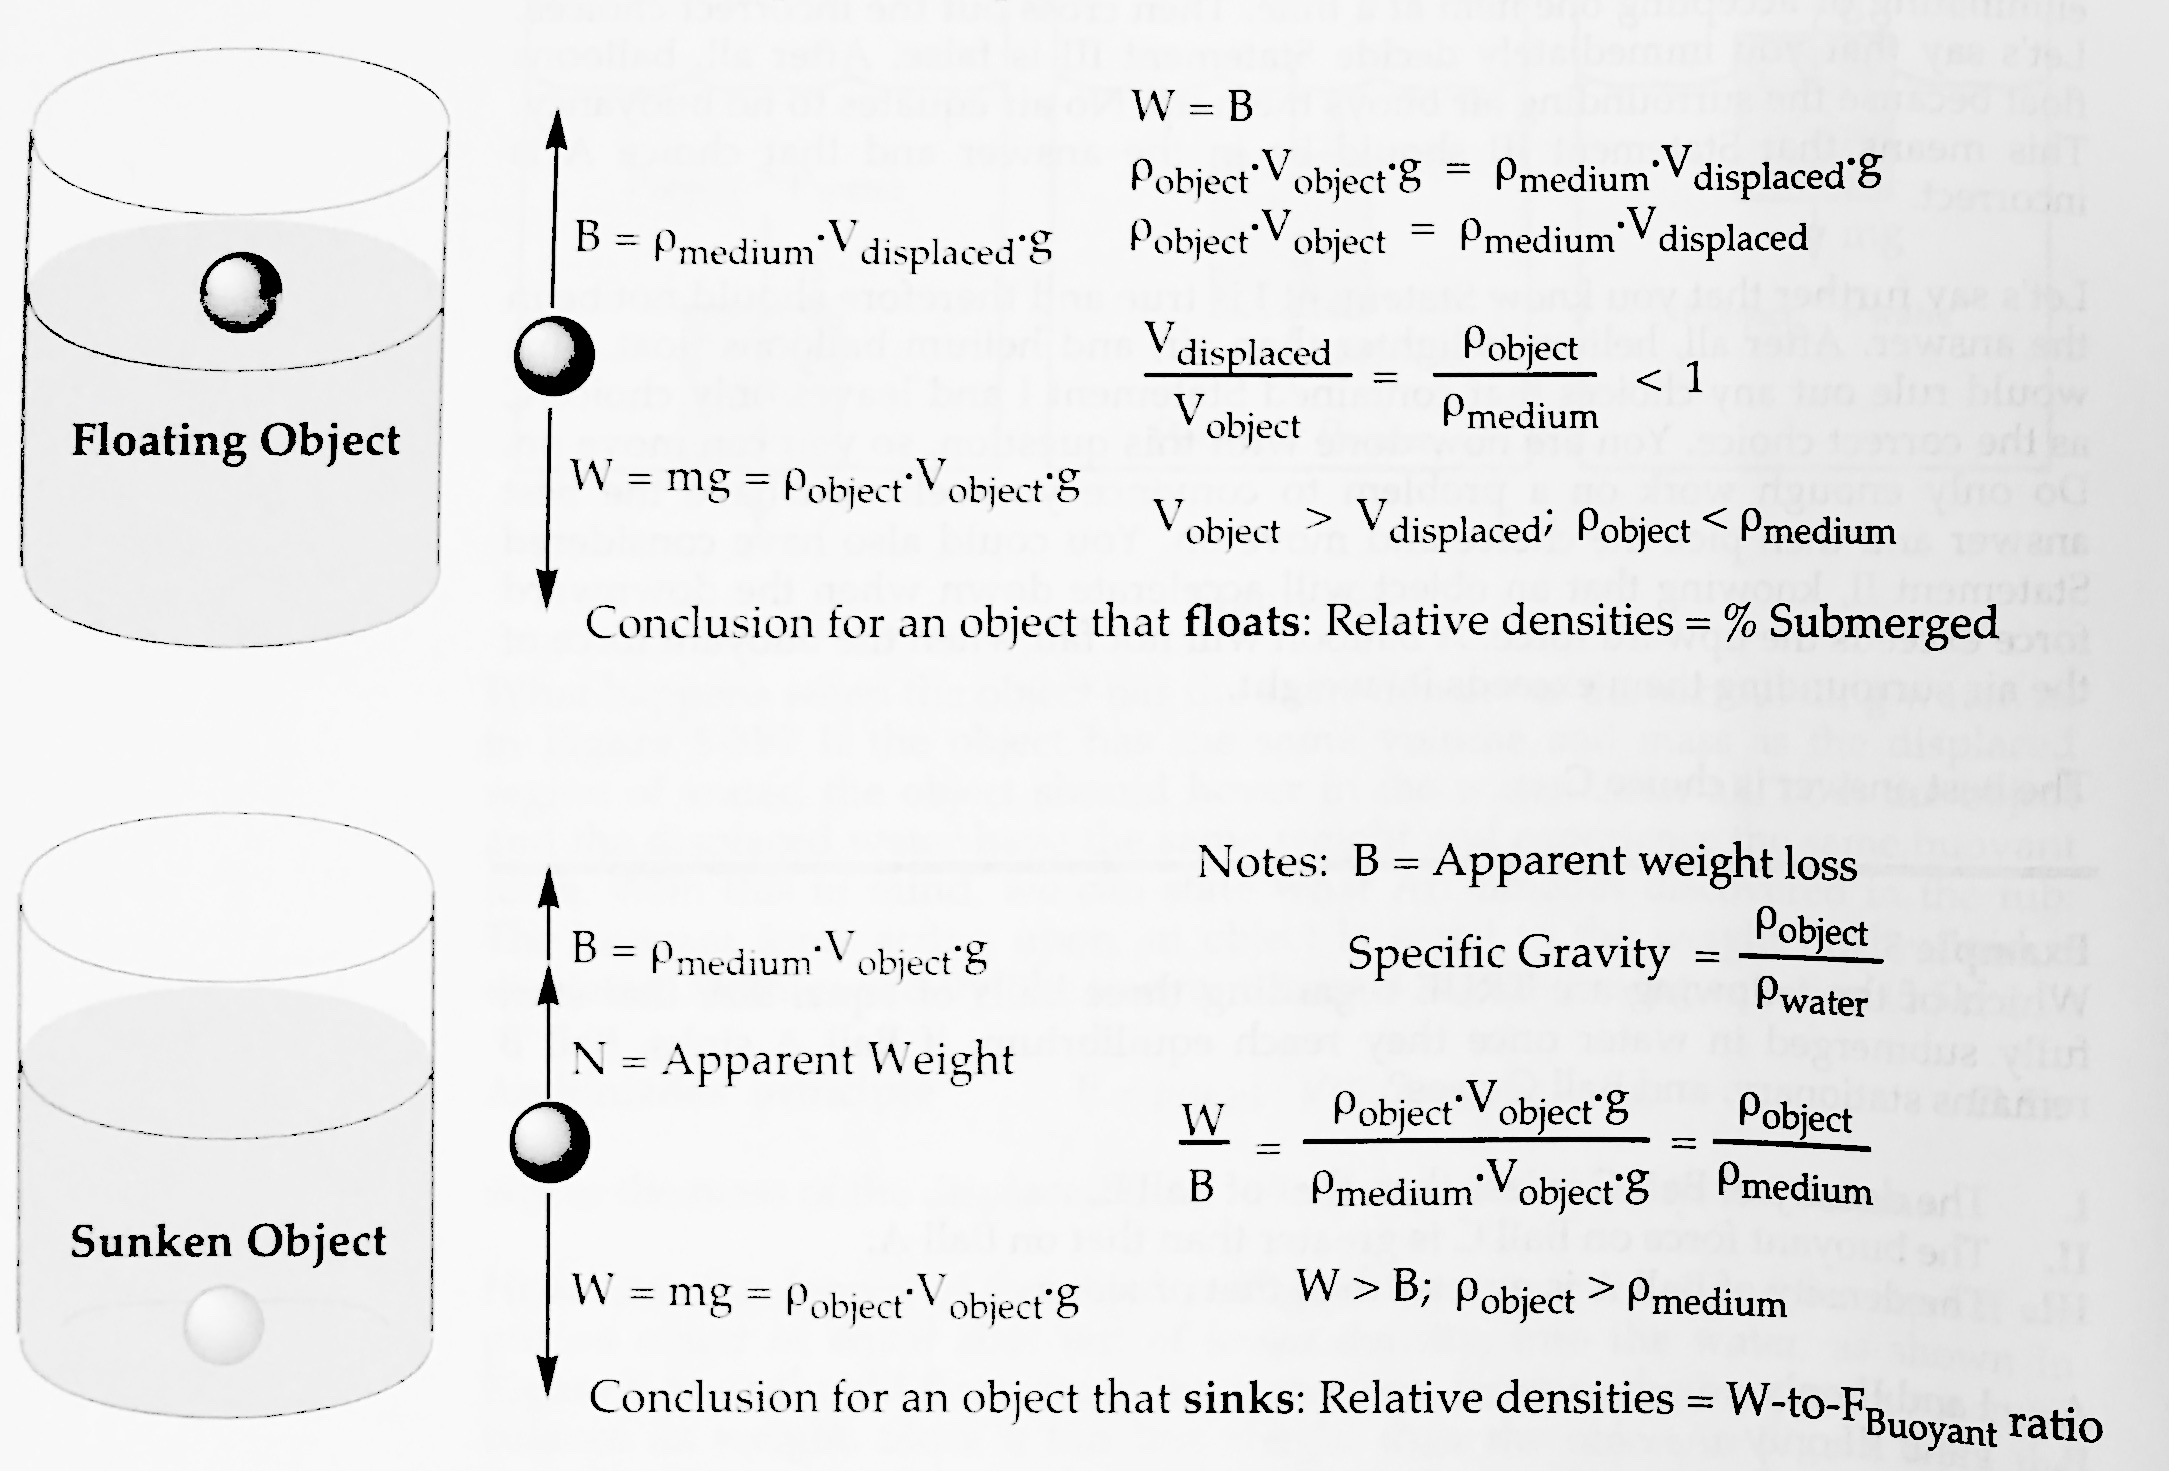
\includegraphics[width=0.8\textwidth]{IMG_3047} \label{3047}
\caption{Mathematics of Objects placed in Tanks of Fluid}
\end{figure}
\noindent Here is an example problem associated with the information shown in \textbf{Figure \ref{3047}}:
\begin{center}
\begin{minipage}{30em}
\textcolor{blue}{What is the specific gravity of an object that weighs 36N in air but only 9N in water at $4^{\circ}$C?
\begin{enumerate}[label=\Alph*]
	\item 0.25
	\item 1.33
	\item 3.00
	\item 4.00
\end{enumerate}}
\end{minipage}
\end{center}
\noindent Because the object still has weight in water, this means that the object is a sunken object rather than a floating object. Thus, the object must be denser than the medium, so the specific gravity must be greater than 1. Based on the given information, the buoyant force must be 27N. Keep in mind that a sunken object rests on the bottom of the container, where because it experiences no acceleration, it has a net force of zero. This means that on the bottom fo the tank, $mg=N+B$, where $N$ is the perceived weight of the object in water, $B$ is the buoyant force, and $mg$ is the actual weight of the object in water. To get the specific gravity (the relative densities), we simply divide 36 by 27:
\begin{equation}
\begin{split}
\text{Specific Gravity}=\frac{W}{B}=\frac{36\text{N}}{27\text{N}}=\frac{4}{3}=1.33
\end{split}
\end{equation}
\noindent Thus, the correct answer is \textbf{B}. \\
\indent The force associated with the tendency of the surface of a liquid to pull inward and shrink in area is known as \textbf{surface tension}. This is largely due to intermolecular forces such as hydrogen bonding or van der Waals interactions. 

\subsection{Viscosity and Poiseuille's Principle}
Friction in fluids is called \textbf{viscosity} ($\eta$), which units of $\text{N}\cdot\text{sec}/\text{m}^2$. Viscous forces retard the motion of one part of a fluid relative to another part of the fluid. If two layers of a fluid are held together tightly, then the viscosity of the fluid is said to be large, and the fluid will move \textit{slowly}. Generally, when the temperature of a fluid \textit{increases}, the viscosity of a liquid would \textbf{decrease} while the viscosity of a gas would \textbf{increase}. When a simple fluid flows through a pipe, the speed of that fluid is greatest at the central axis of the pipe and essentially zero along the walls of the pipe. As a fluid is flowing through the \textbf{center} of a pipe of length $L$ with a certain speed $v$, there is a force that tends to oppose the fluid's motion. That force is called a \textbf{\textit{viscous retarding force}} $F$ and it is caused by the fluid's resistance to flow. The magnitude of $F$ is given by
\begin{equation}
\begin{split}
F=4\pi\eta L v
\end{split}
\end{equation}
\noindent The net force on a fluid is proportional to the difference between the pressures of the pipe at the different ends. For the fluid to flow through the center of the pipe at constant speed, the driving force and the retarding force must be equal. If we substitute the cross sectional area $A=\pi r^2$ for a pipe, then we get
\begin{equation}
\begin{split}
4\pi\eta Lv=A\left(p_1-p_2\right)\longrightarrow v=\left(\frac{p_1-p_2}{4\eta L}\right)r^2
\end{split}
\end{equation}
\indent The \textbf{volume flow rate} $Q$ is the volume $V$ of fluid that passes through a pipe per unit time. Recall that we have mentioned that the fluid in a pipe flows the fastest at the center of the pipe and does not flow at all at the edges of the pip. Using this assumption, we can express the average speed of the fluid as $\bar{v}=v/2$. If we also assume a circular cross-sectional area of $A=\pi r^2$, then we can arrive at $Q=V/t=\left(v/2\right)\pi r^2$. Plugging in the result from earlier for the speed of fluid flow, we arrive at \textbf{Poiseuille's Principle}:
\begin{equation}
\begin{split}
Q=\frac{\pi r^4}{8\eta L}\left(p_1-p_2\right)
\end{split}
\end{equation}
An important parameter in Poiseuille's Principle is the $r^4$ term. Note that if the radius of the pipe is doubled, the flow rate increases by a factor of 16. Although we have presented Poiseuille's Principle as a mathematical expression to this point, at the level of the MCAT it is highly conceptual. For instance, it explains that an extremely tall person will have a greater strain on their hair than a person of average height, because in order to generate the same volume flow rate $Q$, a tall person requires a greater $\Delta p$ to offset the greater $L$ associated with their longer circulatory system.

\subsection{Continuity Equation}
Assuming that fluid is incompressible, at any given moment in time, the fluid entering one region with cross sectional area $A_1$ must equal the fluid leaving the region at $A_2$. In other words, the volume flow rates for the two regions must be equal. This gives us the \textbf{continuity equation}
\begin{equation}
\begin{split}
Q=A_1\bar{v}_1=A_2\bar{v}_2
\end{split}
\end{equation}
\noindent The continuity equation can also apply to branching as long as the fluid is incompressible and that the total cross-sectional areas of all the branches is considered. Here is an example of a problem involving the continuity equation:
\begin{center}
\begin{minipage}{30em}
\textcolor{blue}{Atherosclerosis is the thickening and hardening of the arterial walls. The aorta of a healthy adult has a radius of about 1.3 cm and a blood flow velocity of about 0.5 m/s. An atherosclerosis-stricken bacon epicure is found to have an effective aortic radius that is 75\% of that in a healthy aorta. What is the blood flow velocity through the narrowed section of the artery? (Assume that the blood's volumetric flow rate is constant for all adults.)
\begin{enumerate}[label=\Alph*]
	\item 0.28 m/s
	\item 0.38 m/s
	\item 0.66 m/s
	\item 0.89 m/s
\end{enumerate}}
\end{minipage}
\end{center}
\noindent This problem is easily solved using the continuity equation:
\begin{equation}
\begin{split}
A_1\bar{v}_1=A_2\bar{v}_2\rightarrow\bar{v}_2=\frac{A_1}{A_2}\bar{v}_1=\frac{\pi \left(1.3\text{ cm}\right)^2}{\pi \left(0.75 \cdot 1.3\text{ cm}\right)^2} \left(0.5\text{ m/s}\right)=\frac{16}{9}\frac{1}{2}\text{ m/s}=\frac{8}{9}\text{ m/s}\approx 0.89 \text{ m/s}
\end{split}
\end{equation}
\noindent Therefore, the best answer choice is \textbf{D}. 

\subsection{Bernoulli's Equation}
Bernoulli's Equation stems from the work-energy theorem as applied to a moving fluid system. \hilight{TODO} %TODO

\subsection{Turbulence}
When we looked at Poiseuille's Principle, we say that adjacent layers of a fluid have the ability to slide past one another in a smooth and uniform fashion. This is called \textbf{laminar} flow. Poiseuille's Principle only holds for laminar flow. If the flow of a fluid is sufficiently high, then a chaotic and irregular pattern develops in the fluid\textemdash this is called \textbf{turbulent} flow. Viscous frictional forces increase during turbulent flow.\\
\indent The \textbf{Reynolds number} $N_R$, defined by
\begin{equation}
\begin{split}
N_R=\frac{2\rho\bar{v} R}{\eta}
\end{split}
\end{equation}
\noindent tells us whether flow is laminar or turbulent, where $\rho$ is the density of the fluid, $\eta$ is the viscosity, $\bar{v}$ is the average velocity of the fluid, and $T$ is the radius of the vessel through which the fluid flows. $N_R<2000$ means the flow is laminar, $N_R>3000$ means the flow is turbulent, and anywhere in between means the flow is unstable. This means that flow can be either laminar or turbulent depending on the material. Here's an example of a problem involving turbulence:
\begin{center}
\begin{minipage}{30em}
\textcolor{blue}{Which of the following will decrease the chance of turbulent blood flow in a vein?
\begin{enumerate}[label=\Alph*]
	\item Widening the vein while maintaining the same flow speed.
	\item Thinning the blood without changing its density.
	\item Increasing the absolute pressure on each end of the vein by the same amount.
	\item Lowering the blood density without thinning it.
\end{enumerate}}
\end{minipage}
\end{center}
\noindent Widening the vein increases $R$, which increases the Reynold's number and thus the chance of turbulent flow, so choice A is eliminated. Thinning the blood decreases $\eta$, which increases the Reynold's number and thus the chance of turbulent flow, so choice B is eliminated. Increasing the absolute pressure on each end of the vein doesn't do anything according to the mathematical definition of the Reynold's number, so choice C is eliminated. Lowering the blood density decreases $\rho$, which decreases the Reynold's number and thus the chance of turbulent flow, so choice \textbf{D} is the correct answer.

\section{Biochemistry and Molecular Cell Biology}
\subsection{Amino Acids and Proteins}
All of the standard 20 amino acids are referred to as \textit{$\alpha$-amino acids} (i.e. a 2-amino acid), except for \textit{proline} which is referred to as an \textit{$\alpha$-imino acid}. Configurations (either relative or absolute) in amino acids refers to the stereochemical configuration around the chiral carbon. Due to differences in the priority of different amino acid side chains, not all amino acids have the same ``absolute configuration,'' which refers the R/S naming convention. However, all amino acids have the same ``relative configuration,'' which refers to the D/L naming convention. All biologically produced amino acids are in the L configuration. \\ 
\indent The charged R groups are Asp (aspartate), Glu (glutamate), Lys (lysine), Arg (arginine), and His (histidine). All of these are highly ionized at neutral pH except for His, which is only weakly ionized.\\
\indent Body fluids have pH range from 6.5 to 8.0\textemdash at these ranges, the amino and carboxyl groups are ionized. In other words, the $\alpha$-amino group bears a positive charge, while the $\alpha$-carboxyl group bears a negative charge. This is referred to as the \textbf{zwitterionic} nature of amino acids, due to the fact that the pKa of the $\alpha$-amino terminal is about 9.4, while it is about 2.2 for the $\alpha$-carbxyl terminal. Since amino acids can act as either an acid or a base, they are referred to as \textbf{ampholytes}. To determine the fraction of either the $\alpha$-amino, $\alpha$-carboxyl, or side chain groups that are ionized at a particular pH, use the \textbf{Henderson-Hasselbalch Equation}:
\begin{equation}
\begin{split}
\ce{pH}=\ce{pK_a}+\log\frac{\ce{[A^-]}}{\ce{[HA]}}
\end{split}
\end{equation}
\noindent The \textbf{isoelectric point} is the pH at which an amino acid carries \textbf{no net} electric charge. From the Henderson-Hasselbalch Equation, we know that the isoelectric point pI can be rewritten as
\begin{equation}
\begin{split}
\ce{pI}=\frac{\ce{pK_{a1}+pK_{a2}}}{2}
\end{split}
\end{equation}
\noindent Basically, it's just the main of all of the pKa values associated with the side groups for the molecule. For most amino acids, you only need to factor in the $\alpha$-COOH and $\alpha$-N$\text{H}_3^+$ pKa values, although the R side group may also contribute as well. In terms of making buffers, if a weak acid is within 1 pH unit of its pKa value, it resides within a good buffering range.\\
\indent Polypeptides with a net positive charge at physiologic pH (\textasciitilde7.4) most likely contain amino acids with \textit{basic} R groups. Polypeptides with a net negative charge at physiologic pH most likely contain amino acids with \textit{acidic} R groups. \\
\indent Electrophoretic separation of leucine from a protein sample would be least effective at pH 7.4, as opposed to pH values of 2.4, 1.4, and 0.4, because leucine has an aliphatic side chain, and so at physiological pH, leucine exists as a zwitterion. \\
\indent Formation of \textbf{peptide bonds (peptide linkages)} requires an input of free energy; the hydrolysis of the peptide bond would be more favorable than its synthesis. Remember that peptide unit (i.e. the \ce{O-C-N-H} bonding) is planar due to resonance!\\
\indent The \textbf{central dogma} is essentially that DNA makes RNA makes protein. DNA makes additional DNA via DNA replication, DNA makes RNA via transcription, and RNA makes protein via translation; this has typically been the canonical view of how information flows in biological systems. However, there are other pathways as well\textemdash RNA can make cDNA via reverse transcription (common in retroviruses such as HIV), and there are also ncRNAs (noncoding RNAs) that can directly perform functions within the cell as an RNA molecule. Two examples of ncRNAs are tRNAs (transfer RNAs) and rRNAs (ribosomal RNAs), both of which are used for the translation of mRNAs into proteins. \\
\hilight{Still need to write notes for peptide bonds: formation and cleavage on Khan academy}\\ %TODO
\indent There are a total of 20 canonical amino acids, shown in Figure \ref{Amino_Acids}. Make sure to memorize all of them. There are four amino acids in particular that are worth talking about due to their individual special properties\textemdash histidine, proline, glycine, and cysteine.
\begin{enumerate}
	\item Histidine is a special residue because its R group has a pKa of about 6.5, which is pretty close to the physiological pH of 7.4. Recall that at pH less than an amino acid's pKa, the amino acid exists in a protonated (positively charged form), and at pH greater than an amino acid's pKa, it will exist in the deprotonated form. Because histidine is in that `special' regime, histidine is going to exist in both the protonated and deprotonated forms. So, this makes it a particularly useful amino acid to have at the active site of a protein where it can both stabilize or destabilize a substrate.
	\item Proline has a secondary $\alpha$ amino group. All this basically means is that the side chain forms a second bond with the $\alpha$ nitrogen of this amino acid. Because of this unique cyclic structure of proline, this amino acid plays a central role in the formation of $\alpha$ helices and $\beta$ sheets secondary structures. More specifically, it disrupts $\alpha$ helices because of the secondary $\alpha$ amino group, thus introducing kinks into $\alpha$ helices. Proline is thus an \textit{$\alpha$ helix breaker}.
	\item Glycine has just one hydrogen atom as its side chain. Because of this, the central carbon is now achiral (the only amino acid to be non-optically active. Additionally, because of the small R group, glycine is very flexible, so there's a lot of free rotation around the $\alpha$ carbon. Glycine also disrupts $\alpha$ helices because of its enhanced flexibility, thus also introducing kinks into $\alpha$ helices, and is thus also an \textit{$\alpha$ helix breaker}. 
	\item Cysteine has a special thiol \ce{-SH} group as its R group, meaning that when two cysteine residues are in close proximity, then their side chains can form an \ce{S-S} bond called a \textit{disulfide bridge}. Disulfide bridges exist in oxidizing environments, because the normal thiol groups exists in the reduced form in a reducing environment. For example, the extracellular space is an oxidizing environment, so this will favor the formation of disulfide bridges. However, in the cytosol (which is a reducing environment), disulfide bridges will likely not form. 
\end{enumerate}
\begin{figure}[h!]
\centering
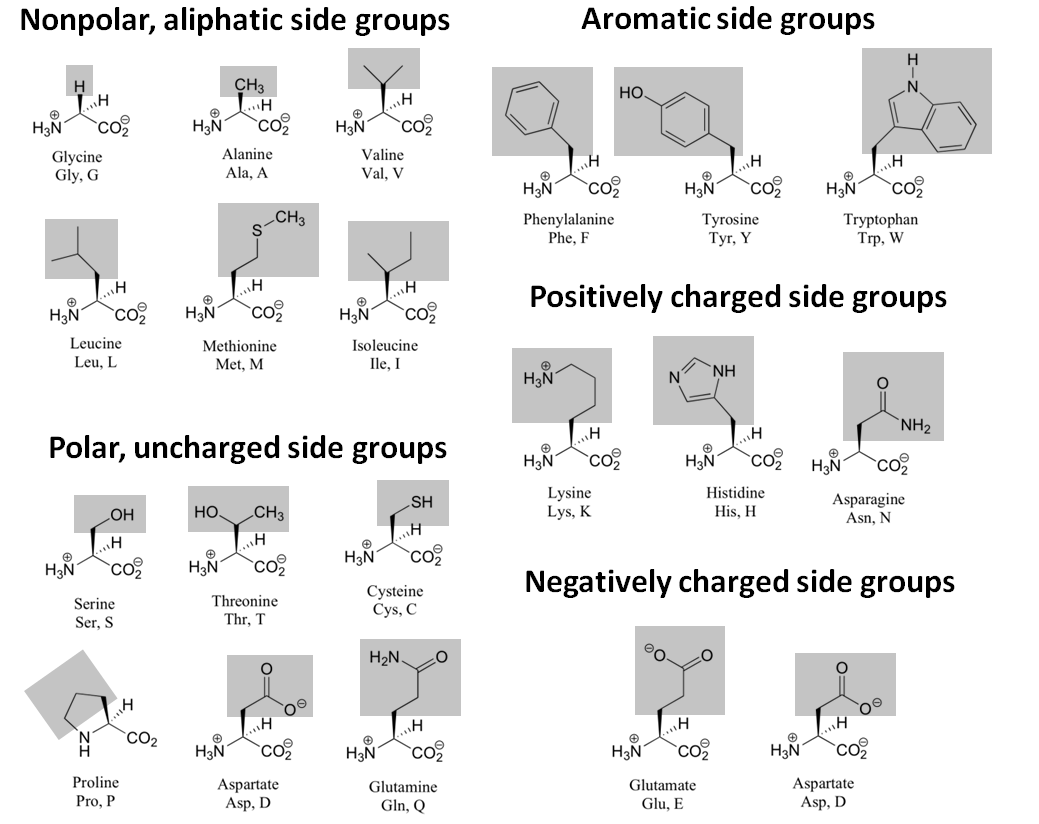
\includegraphics[width=0.8\textwidth]{Amino_Acids.png} \label{Amino_Acids}
\caption{20 Canonical Amino Acids, all with L configuration}
\end{figure}

\subsection{Carbohydrates \& Lipids}
Carboyhydrates have an empirical formula \ce{(CH_2O)_n}. They also must have an \textit{aldehyde} or \textit{ketone} functional group and at least \textit{two} alcohol functional groups. If a carbohydrate contains an aldehyde, it is referred to as an \textbf{aldose}. If it contains a ketone, it is referred to as a \textbf{ketose}. 

\subsection{D- and L- Isomers}
In Fischer projections, we care about the chiral carbon that is most distant from the carbonyl carbon. This chiral carbon is referred to as the \textbf{reference carbon}. If the hydroxyl group attached to that reference carbon is to the right, the molecule is the \textbf{D isomer}. If the hydroxyl group is to the left, the molecule is the \textbf{L isomer}. Most of the naturally occurring sugars are found in their D form (while most of the naturally occurring amino acids are found in their L form).

\subsection{Monosaccharides, Oligosaccharides, and Polysaccharides}
Sugars with five or more carbon atoms in their backbone prefer to be in the cyclic form. The C-1 carbon is the carbonyl carbon, also called the \textbf{anomeric carbon}. Two diastereomers of cyclic monosaccharides are $\alpha$ and $\beta$. In the $\alpha$-anomer, the \ce{-OH} group at the anomeric carbon is on the \textit{opposite} side of the ring from the \ce{-CH_2OH} group that is attached to the reference carbon. In the $\beta$-anomer, the \ce{-OH} group at the anomeric carbon is on the \textit{same} side of the ring as the \ce{-CH_2OH} group that is attached to the reference carbon. An example of anomers is shown in Fig. \ref{anomers}. Notice that, depending on the starting sugar, formation of the cyclic ring creates either a \textit{hemiacetal} group or a \textit{hemiketal} group. 
\begin{figure}[h!]
\centering
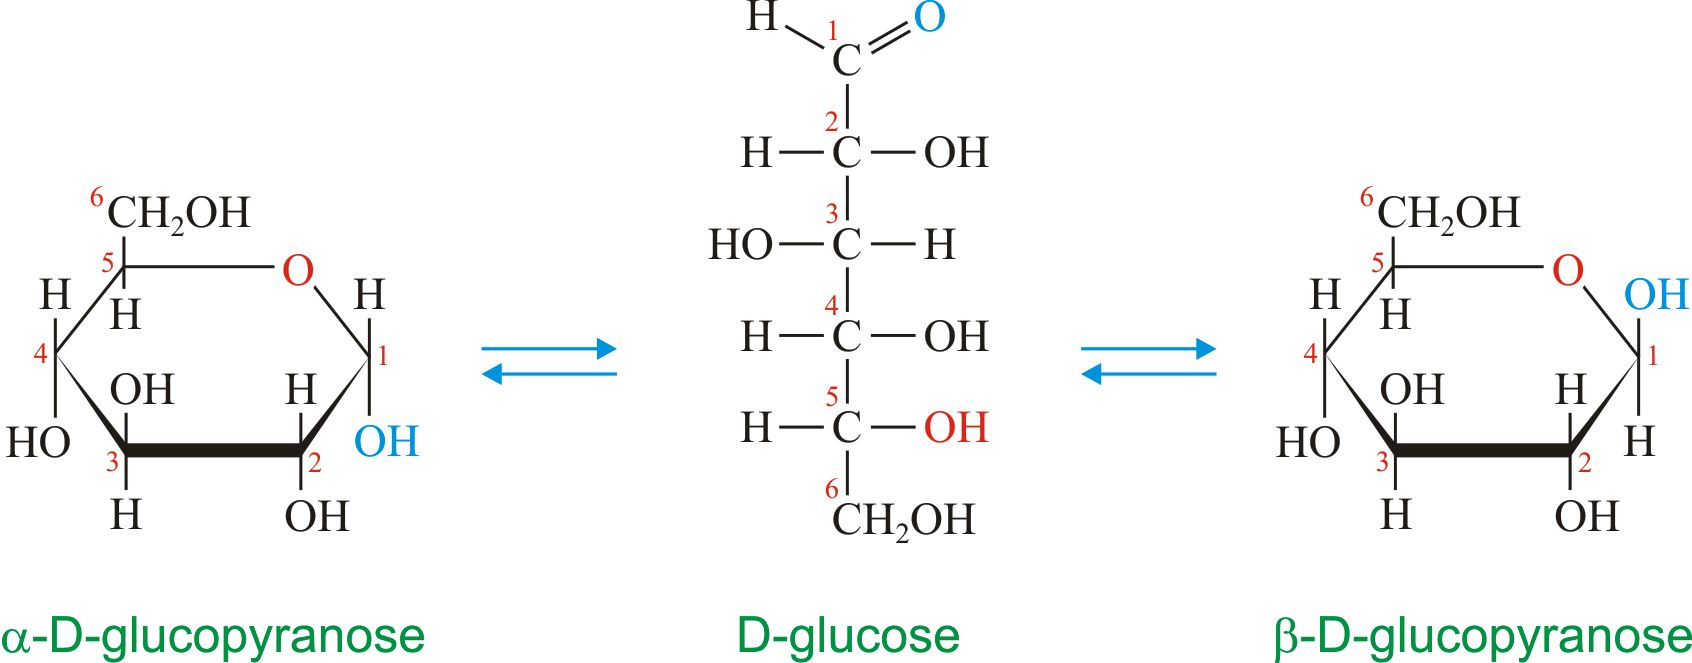
\includegraphics[width=0.8\textwidth]{anomers.png} \label{anomers}
\caption{Formation of the two anomers of D-Glucopyranose}
\end{figure}
\indent Two oxidizing agents used to identify the functional groups of carbohydrates are \textbf{Tollens' reagent} (which contains \ce{Ag^+}) and \textbf{Benedict's reagent} (which contains \ce{Cu^{2+}}). If an aldose or ketose is capable of reducing these ions, those sugars are referred to as \textit{reducing sugars}. Reducing sugars have the suffix \textbf{-ose}, while non-reducing sugars have the suffix \textbf{-ide}. Carbohydrates that contain a hemiacetal or a hemiketal group give positive tests with Tollens' and Benedict's reagents.\\
\indent A sugar is a non-reducing sugar if its hemiacetal or hemiketal group has been converted to an acetal or ketal group, respectively (i.e. through reacting with an alcohol). These non-reducing sugars will not react with either the Tollens' reagent or Benedict's reagent. \\
\indent The structure of lactose disaccharide has been given on the MCAT a number of times. Two important storage polysaccharids are \textit{starch} and \textit{glycogen}. Starch is a food reserve in plants. It is basically a bunch of D-glucose molecules linked together primarily with $\alpha\left(1\rightarrow 4\right)$ linkages, although there can be other types depending on the type of starch. Glycogen is the storage polysaccharide common to all animals, and is located primarily in skeletal muscle and liver tissue.

\subsection{Lipids}
Fatty acids are carboxylic acids with a hydrocarbon side chain. They can be either saturated or unsaturated. In nature, fatty acids are rarely free. Rather, they are esterified to a glycerol backbone to form a \textit{triacylglycerol}. There are a number of different types of lipids that we will discuss here:
\begin{enumerate}
	\item \textbf{Glycerophospholipids} (or phosphoglycerides) are the ones that we're most familiar with\textemdash two fatty acids esterified to the C-1 and C-2 carbons of glycerol, and a phosphate group attached to C-3. These molecules are amphiphilic, as they have nonpolar tails and a polar head.
	\item \textbf{Sphingolipids} do not have a glycerol backbone, and instead are derivatives of amino alcohols. The C-2 carbon has an amino group, and a fatty acid can be attached to it as well through an amide linkage\textemdash this molecule is called a \textit{ceramide}. Sphingomyelins are special types of sphingolipids that have a phosphoethanolamine or phosphocholine group attached to the C-1 carbon of the ceramide, and are abundant in the myelin sheaths that surround the axons of nerve cells.
	\item \textbf{Cholesterols} are synthesized in the cytosol. Steroids are based on cholesterols and synthesized in the mitochondria. Cholesterol is transported into the mitochondrion, and adrenocorticotropic hormone (ACTH) stimulates the conversion of cholesterol to pregnenolone. The five types of steroid classes are progesterone, glucocorticoids, mineralocorticoids, androgens, and estrogens.
\end{enumerate}
\noindent Cholesterol becomes pregnenolone, which then becomes progesterone. Progesterone can then either become testosterone, aldosterone, or cortisol. Testosterone can be further converted into estradiol. Progesterone is important for women to maintain pregnancy and the endometrial lining of the uterus, although it is also found in low levels in males. Cortisol (also known as hydrocortisone) is synthesized and secreted from cells in the cortex of the adrenal glands. In the liver, cortisol increases both glycogen synthesis and gluconeogenesis. In skeletal muscle, cortisol decreases glucose uptake and protein synthesis, and increases protein catabolism. In adipose tissue, cortisol increases lipid mobilization and decreases glucose uptake. Aldosterone is synthesized and released from cells in the adrenal cortex. It increases reabsorption of sodium ions in the kidneys, intestines, salivary glands, and sweat glands. This leads to retention of sodium in the extracellular fluid (ECF), thus increasing ECF volume, blood volume, blood pressure, and blood flow. Testosterone is important for sperm maturation in males and development of secondary sex characteristics. Estradiol is the primary estrogen in women and is important in the development of secondary sex characteristics and regulation of the ovarian cycle. \\
\indent Cholesterol decreases membrane fluidity at high temperatures and increases membrane fluidity at low temperatures. Basically, the way to remember this is that whatever the thermodynamically expected behavior of the cell fluidity is at a given temperature, cholesterol decreases the magnitude of that effect so that the membrane behavior never gets too extreme.\\
\indent In order to tolerate high temperatures, a thermophilic bacterium must have fatty acid tails that decrease the fluidity of its cell membrane. Saturated fatty acid tails have stronger Van der Waals interactions and thereby decrease the fluidity of cell membranes. Longer fatty acid tails have greater surface area for Van der Waals interactions, so they also decrease the fluidity of cell membranes. Therefore, long saturated hydrocarbon tails would best help the thermophilic bacteria have stable plasma membranes.\\
\indent Pinocytosis is the ingestion of liquid into a cell by the budding of small vesicles from the cell membrane.

\subsection{Cellular Reproduction and Chromosomes\textemdash Eukaryotic Cells}
\textbf{Chromatin} is a complex of dsDNA and histones (which are a type of protein). Histones are basic proteins consisting of a high percentage of Lys and Arg residues that bear of a positive charge. This allows them to easily establish a favorable electrostatic relationship with the negatively charged DNA polymers. There are also nonhistone proteins (i.e. RNA polymerase) that are acidic and bear a net negative charge. Chromatin condenses into \textbf{chromosomes} as the cell prepares for division. At metaphase, each chromosome consists of two \textbf{sister chromatids}, each held together through a constricted region called the \textbf{centromere}. \\
\indent There are five types of histones: H1, H2A, H2B, H3, and H4. A nucleosome is an association of these histones with a specific length of DNA. H2A, H2B, H3, and H4 are the \textbf{core} histones. The H1 histone is thought to play an important role in pulling the individual nucleosomes together to help with DNA condensation. 
\begin{figure}[h!]
\centering
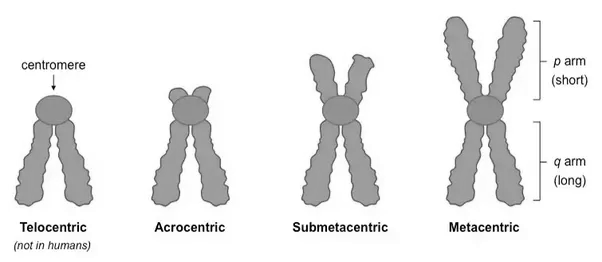
\includegraphics[width=0.65\textwidth]{chromosome_types.png} \label{chromosome_types}
\caption{General classification of eukaryotic chromosomes based on the position of the centromere.}
\end{figure}
Mitosis should honestly be pretty straightforward. The only thing is that for prophase, there may be some new terminology. At the beginning of prophase, the two \textbf{centriole} pairs begin to move apart, and microtubules begin to radiate from each pair in all directions, forming a star-like structure called an \textbf{aster}. The region from which the microtubules extend outward is called the \textbf{centrosome}, or MTOC (microtubule-organizing center). The microtubules ultimately form the \textbf{mitotic spindle}, and attach to the chromosomes at the \textbf{kinetochore}, a specialized area closely associated with the centromere.

\subsection{Meiosis}
Meiosis is technically composed of two processes\textemdash Meiosis I and Meiosis II\textemdash each of which s preceded by an interphase. During the second interphase immediately before meiosis II, the S period does not exist and so the DNA cannot be replicated again. Meiosis is a bit more complicated than mitosis, so let's take a look at it step by step:
\begin{itemize}
	\item Prophase I is longer and more complicated to prophase of mitosis, and can be divided into five stages: leptotene, zygotene, pachytene, diplotene, and diakinesis. During \textit{leptotene}, the replicated chromosomes have already started to condense and now become visible. During \textit{zygotene}, the synaptonemal complex forms where the maternal and paternal chromosomes come together to form the tetrads. This is in preparation for crossing over, although crossing over has not occurred yet. At this stage, there are 23 tetrads, 2 centromeres in each tetrad, and 46 chromosomes (based on the number of centromeres). During \textit{pachytene}, chromosomes continue to condense, and crossing over occurs. During \textit{diplotene}, the homologous chromosomes begin to separate and the events of crossing over become visible at structures called \textbf{chiasmata}. During \textit{diakinesis}, the nuclear envelope begins to break down, and the nucleoli disappear. 
	\item Metaphase I is unremarkable.
	\item During Anaphase I, the microtubules pull the homologous chromosomes apart, but the centromeres do \textit{not} divide. Each chromosome that migrates toward a pole is still composed of sister chromatids, and this pair is referred to as a \textbf{dyad}. Cytokinesis also begins at this step.
	\item Telophase I and Cytokinesis are unremarkable. After the completion of Meiosis I, we find that a diploid cell with 46 chromosomes has divided into two haploid cells, each with 23 chromosomes. This is therefore a \textbf{reductive division}.
	\item Interphase II is usually pretty brief.
	\item Meiosis II is pretty unremarkable. One thing to note is that the cells entering Meiosis II are already haploids. Also, because of the crossing over events from Meiosis I, the chromatids of each chromosome that are separating during Anaphase II can't actually be referred to as \textit{sister} chromatids because their DNA is no longer the same because of the genetic recombination.
\end{itemize}
\noindent Yeast are an example of a eukaryote that reproduces asexually.

\subsection{Biomembranes and Membrane Transport}
In lipid bilayers, recall that lateral diffusion of neighboring phospholipids is very common, but transverse diffusion (flip-flop) of phospholipids from one lipid plane to the next is a very rare event. Addition of cholesterol to a membrane acts to decrease fluidity, as the planar steroid ring inserts between neighboring fatty acid side chains and interferes with the movement of those chains. It might be a good idea to review that one problem about the symports and antiports from the Bi9 Final. \\
\indent There's also something called \textbf{group translocation} found in certain bacteria, where a sugar residue like glucose is phosphorylated as it is being transported through the plasma membrane. This type of transport is coupled to cellular metabolism. There's also \textbf{bulk transport} that involves \textit{indosomes} and \textit{endocytotic vesicles}. Many animal cells will show an invagination of a portion of their plasma membrane that will eventually pinch off to form an internalized vesicle. Bulk transport is where words like endocytosis, pinocytosis, phagocytosis, and exocytosis come in.

\subsection{Nucleus, Nucleolus, \& Ribosomes}
The nucleus is double membrane-bound. The outer membrane is actually considered to become part of the rough endoplasmic reticulum (RER). Between the inner and outer membrane is the \textbf{perinuclear space}. DNA replication and transcription occur in the nucleus, while translation happens outside in the cytosol. The diameter of \textbf{nuclear pores} is 10-20 nm. \\
\indent Within the nucleus is a highly organized region called the \textbf{nucleolus}. The nucleolus is \textit{not} a membrane-bound organelle. It is centered around certain chromosomes that contain \textit{nucleolus organizer regions}, and is involved in the synthesis of rRNA. If a cell is quite actively involved in protein synthesis (meaning that it needs a lot of rRNA), one would expect the nucleolus to be larger than if a cell were not as actively involved in protein synthesis. \\
\indent Eukaryotic ribosomes are composed to two subunits, each differing in size and content of RNA and protein. We talk about ribosome size based on a sedimentation coefficient called the \textbf{Svedberg unit (S)}, where one S $=10^{-13}$ sec. The rate at which a molecule sediments in an ultracentrifuge tells us something about its mass. The sedimentation coefficient of a complete eukaryotic ribosome is expressed as \textbf{80S}. Eukaryotic ribosomes have two subunits\textemdash a large subunit (60S) and a small subunit (40S). Note that 60S + 40S $\neq$ 100S; in other words, the values are not additive. Sedimentation coefficients are not linearly related to molecular weight, as they depend on the size and the shape of the molecule. \\
\indent The overall dimensions of a complete ribosome is about $\text{\textbf{20 nm}}\times\text{\textbf{30 nm}}$, and contains roughly 60\% rRNA and 40\% protein. The small subunit is about 9 nm in diameter and contains roughly half rRNA and half protein. The large subunit is roughly 25 nm in diameter and contains about 65\% rRNA and 35\% protein. \\
\indent Ribosomes are also found in the matrix of the mitochondria. Ribosomes found in the mitochondrial matrix differn in RNA and protein content, and are also smaller and sediment at about \textbf{55S}. Prokaryotic ribosomes are about \textbf{70S}. 

\subsection{Endoplasmic Reticulum, Golgi Apparatus, \& Lysosomes}
The ER is the largest membrane system in a eukaryotic cell. The \textbf{Smooth Endoplasmic Reticulum (SER)} is tubular in shape and is involved in the synthesis of a majority of the cell's membrane lipids (i.e. neutral fats, phospholipids, prostaglandins, and steroid hormones). Especially in hepatocytes (liver cells), the SER is involved in hydroxylation reactions that aid in the detoxification of drugs by making them more water soluble. The SER can also help catabolize liver glycogen in hepatocytes.\\
\indent The \textbf{Rough Endoplasmic Reticulum (RER)} is flat and sheet-like, and ribosomes on the cytoplasmic fact of the RER are bound to the membrane by their large (60S) subunit. Post-translational modification of proteins occur in the ER lumen, where certain amino acids are modified by hydroxylation and glycosylation events. \\
\indent For the Golgi Apparatus, the \textbf{cis} cisterna face the nucleus/ER, while the \textbf{trans} cisterna face the plasma membrane. The \textbf{medial} cisterna are located between the cis and trans cisternae. After a protein enters the cis cisterna and before it leaves the trans cisterna, it can be modified in a variety of different ways, including glycosylation, sulfation, and proteolysis.\\
\indent Lysosomes contain special enzymes that function at acidic pH values, and are referred to as \textbf{acid hydrolases}, which catalyze the general reaction \ce{A-B + H_2O -> A-H + B-OH}. There are some common acid hydrolases that you should know:
\begin{table}[h!]
\begin{tabular}{llll}
\hline
\textbf{Enzyme} & \textbf{Substrate} & \textbf{Bond Hydrolyzed} & \textbf{Example} \\
\hline
Proteases & Peptides & Peptide & Pepsidase\\
Glycosidase & Glycolipids & Glycoside & $\beta$-hexosaminidase\\
Lipase & Phospholipids  & Carboxylic Ester & Phospholipase\\
Nuclease & DNA & Phosphoric Diester & Acid Deoxyribonuclease\\
Phosphatases & Phosphomonoesters & Phosphoric Monoester & Acid Phosphatase\\
\hline      
\end{tabular}
\end{table}
\noindent Lysosomal enzymes are inactive at neutral pH. The hydrolysis products simply diffuse out of the organelle and are utilized in a variety of metabolic processes. We know that if this were not the case, the increasing solute concentration in the lysosome would eventually result in the lysis of the lysosome due to osmotic water entry into the lysosome, but this is not observed. \\
\indent Peroxisomes are membrane-bound organelles that have a number of enzymes, the most notable being \textit{catalase} that catalyzes the degradation of hydrogen peroxide \ce{H_2O_2}.

\subsection{Signal Hypothesis}
The Signal Hypothesis was covered in Bi9, and is import for co-translational transport. Many proteins have a signal sequence that binds to a signal recognition particle (SRP) in the cytoplasm, halting translation. The SRP chaperones the complex to the signal sequence receptor embedded in the membrane of the RER, and the signal sequence is cleaved by signal pepsidase. Translation then continues and at the same time, the polypeptide chain is transported into the ER lumen via Sec61. 

\subsection{Cytoskeleton}
\textbf{Microtubules} are composed of 13 protofilaments and are about 25 nm in diameter. Each protofilament has alternating $\alpha$-tubulin and $\beta$-tubulin proteins. The growth of microtubules occurs from \textbf{microtubule organizing centers (MTOCs)}. Three common centers are the centrosome (cell center), kinetochores (spindle attachment sites on chromosomes), and centrioles. Polymerization preferentially occurs at the (+) end.\\
\indent \textbf{Microfilaments} (actin filaments) are about 7 nm in diameter. Polymerization preferentially occurs at the (+) end. We have G-actin (globular) monomers, and F-actin (filamentous) polymerized subunits. \\
\indent \textbf{Intermediate filaments} are about 8 to 12 nm in diameter and differ in composition. For example, the intermediate filaments in epithelial cells are composed of keratins, while in muscle cells they are composed of desmin. 

\subsection{Prokaryotic Cells}
The two most frequently encountered bacteria are the \textbf{cocci} and the \textbf{rods}. Cocci are essentially spherical in shape while rods generally resemble the shape of a tube. Bacteria that have a rigid twist to their rod-like structure are called \textbf{spirilla}. If their twisted structure is more flexible, they are called \textbf{spirochetes}. Invaginations of bacterial cell membranes are called \textbf{mesosomes} with currently unknown function. \\
\indent Instead of membrane-bound organelles, prokaryotes often have structures called \textbf{inclusion bodies}, which can contain organic molecules like glycogen or inorganic molecules like phosphate granules. Prokaryotic ribosomes are \textbf{70S}, and are composed of a large \textbf{50S} subunit and a small \textbf{30S} subunit.\\
\textbf{Gram positive} bacteria have a rather thick, homogeneous \textbf{peptidoglycan} layer (20 nm to 80 nm) just outside their plasma membrane. \textbf{Gram negative} bacteria have a much thinner peptidoglycan layer (1 nm to 3 nm), in addition to an outer membrane that contains \textbf{lipopolysaccarides} and \textbf{porins}. The polysaccharide helps to stabilize the membrane, and also acts as an \textit{endotoxin} and provides a defense mechanism for the cell. \\
\indent Genetic material can be passed from one bacterial cell to the next by binary fission, bacterial conjugation, transformation, or transduction. Binary fission is basically asexual reproduction where one cell splits into two. In bacterial conjugation, genetic information is transferred by cell-cell contact. Donor strains of bacteria are $F^+$ (male), while the recipient bacteria are $F^-$ (female). The "$F$" refers to the \textbf{fertility plasmid}. Transformation is the uptake of genetic material from the surrounding medium. Transduction is the transfer of bacterial genes by viruses.

\subsection{Viruses}
The architecture of a virus is usually based on one of two structural motifs: \textbf{isometric} (usually in the form of an icosahedron) and \textbf{helical}. The viral protein coat is formed from \textbf{capsomers}. If there is no nucleic acid within the protein coat/shell, then the empty shell is referred to as a \textbf{capsid}. However, if there is nucleic acid within the protein shell, the complex is called a \textbf{nucleocapsid}.\\
\indent The genetic information within the genome of a virus may be encoded in either the language of DNA or RNA, and can be linear or circular, single- or double- stranded, and even segmented. However, no matter how the genetic information is stored in the virus, the translational process uses mRNA as a template. Therefore, by convention, we define that mRNA as being a \textbf{positive (+) strand} nucleic acid.\\
\indent Naked (non-enveloped) viruses gain access to the host's cytoplasm only by receptor-mediated endocytosis. The receptors on the cell surface of the host are usually located near specialized depressions called \textbf{\textit{clathrin-coated pits}}. Enveloped viruses can either enter through receptor-mediated endocytosis or by direct fusion with the plasma membrane. Release of viruses (whether naked or not) is mediated by pH changes, as the pH becomes more acidic in the endosome. 

\subsection{Genetic Information\textemdash Classical Genetics}
Mendel's First Law of Heredity (also called the \textbf{Law of Segregation}) is that alternative alleles segregate from each other in heterozygous individuals and retain their identity. Mendel's Second Law of Heredity (also called the \textbf{Law of Independent Assortment}) is that the hereditary factors (i.e. genes) for different things assort independently of one another. Note that independent assortment of the genes will occur if they are located on different chromosomes or are far apart on the same chromosome.

\subsection{Genetic Loci \& Alleles}
\textbf{Tryptophan} is considered an \textbf{essential amino acid} because it is an amino acid that an organism cannot synthesize itself, and therefore must be obtained from the diet. An \textit{auxotroph} is a mutant that will grow only when its medium is supplemented with a particular compound which is not required by the normal wild type organism. The wild type organism is referred to as a \textit{prototroph}. By definition, an auxotroph will not grow on a minimal medium, while a prototroph will. \\
\indent \textbf{Pleiotropy} is when an individual allele has more than one effect on the phenotype (i.e. there's a mouse gene that determines both the fur coat color and the viability of the mouse). \textbf{Epistasis} is when multiple genes all contribute to a particular phenotype and are able to interact with one another. This occurs between different pairs of genes, \textit{not} between two members of an allelic pair. For example, in order for tryptophan to be synthesized, the dominant allele of all the genes involved in this biosynthetic pathway must be present (in the absence of tryptophan), so the genes involved in the biosynthetic pathway of tryptophan are said to act in an epistatic fashion.\\
\indent The short arm of a chromosome is called the $p$ arm, while the long arm of a chromosome is called the $q$ arm. 

\subsection{Pedigrees \& DNA}
In pedigree charts, males are squares and females are circles. If a square or a circle is filled in with a dark color, then that individual is affected with a given defect. If there is only one copy of any chromosome (i.e. \textbf{monosomy}), the individual will not survive development. The most common form of \textbf{trisomy} is for chromosome 21, which leads to Down's syndrome. It is an example of \textbf{aneuploidy} (the condition in which nuclei have an unbalanced set of chromosomes\textemdash that is, they do not contain an exact multiple of the haploid number of chromosomes). \\
\indent Double stranded DNA has a lower absorbance (by about 40 to 50\%) than single stranded DNA. Also, GC-rich DNA has a lower absorbance than AT-rich DNA at a given temperature. DNA replication is \textbf{semiconservative}. Adenine and guanine are purines (two rings in their structures), while thymine and cytosine are pyrimidines (one ring in their structures). Double stranded DNA is a right-handed helix.

\subsection{DNA Synthesis}
All of the dNTPs have a deoxyribose sugar backbone ($\beta$-D-2'-Deoxyribose) with an N-glycosidic linkage from the C-1 carbon to the purine or pyrimidine. There's also a phophomonoester linkage from the phosphate group to C-4 carbon of the sugar backbone, and additional phosphate groups can chain together via acid anhydride linkages. All dNTPs have 3 phosphate groups chained together. \textbf{DNA polymerase I} adds about 20 dNTP residues to the 3'-hydroxyl function of a pre-existing DNA strand. The dNTPS are added to the newly synthesized DNA chain in the $5'\rightarrow3'$ direction, which means the DNA template is read in the $3'\rightarrow5'$ direction. \\
\indent There are a couple different types of DNA structures that are helices: A-DNA, B-DNA, and Z-DNA. These aren't really important, just know that the canonical DNA form that we're all familiar with is the \textbf{B-DNA} with the major and minor grooves. In A-DNA, $\beta$-D-2-Deoxyribofuranose ring can pucker, and the minor groove essentially vanishes due to the puckering of the furanose ring. The type of helix that is found in A-DNA is also found in regions of double stranded RNA (e.g. involving hairpins) and in RNA-DNA hybrids. Z-DNA is actually a left-handed helix, and involves the phosphates in the backbone zigzagging due to a repeating dinucleotide unit, as opposed to a mononucleotide unit. In Z-DNA, when the pyrimidine bases and the ribose units are far apart, it is in an \textbf{anti} conformation, while it is in a \textbf{syn} conformation when the purine bases and the ribose units are close together.\\
\indent Positive supercoiling is twisting a DNA molecule around its own axis in the right-handed direction, while negative supercoiling is twisting a DNA molecule around its own axis in the left-handed direction (these conventions are for right-handed DNA). The number of times that one DNA strand can be wound around another DNA strand is referred to as its \textbf{linking number (L)}. \textbf{Topoisomers} are DNA molecules that differ only in their linking number. The degree of the linking number in DNA can be altered by enzymes called \textbf{topoisomerases}. \textbf{Type I} topoisomerases reversibly cleave \textit{one strand of DNA} and relaxes negatively supercoiled DNA, while \textbf{Type II} topoisomerases (e.g. DNA gyrase) reversibly cleaves \textit{both strands of DNA} and adds negative supercoils. Negatively supercoiled DNA prepares the DnA duplex for processes like replication, recombination, and transcription where the separation fo the two helical strands is required. \\
\indent The DNA replication process is very systematic. The synthesis of new daughter DNA is coupled to the unwinding of parental DNA at sites called \textbf{replication forks}, which occur at sites referred to as \textbf{origins} (ori for short). In order for the DNA double helix to unwind, \textbf{DNA gyrase} adds negative supercoils ahead of the advancing replication fork, as when the replication fork is initially unwound, positive supercoils are introduced making DNA separation rather difficult without the DNA gyrase activity. \textbf{Helicase} then binds to the ori site and catalyzes the ATP-driven unwinding of the duplex DNA. Single-stranded binding proteins then stabilize the unwound portion of the parental DNA. \\
\indent From here, both strands can serve as template strands, but DNA Polymerase I can only synthesize DNA in the $5'\rightarrow3'$ direction. We therefore have a leading strand with continuous replication, and also a lagging strand that uses \textbf{Okazaki fragments} to discontinuously synthesize the complementary strand (the primers used are RNA primers). DNA Polymerase III holoenzyme is used to synthesize the lagging strand (as opposed to DNA Polymerase I) because it is quicker and can add more dNTP's to the growing DNA strand. DNA polymerase I also has $5'\rightarrow3'$ exonuclease activity that allows it to remove the short segments of RNA primer, and then add deoxyribonucleotides to the free $3'$-hydroxyl function of the chain undergoing elongation. \textbf{DNA ligase} then joins together the Okazaki fragments. It is important to remember that replication of DNA can be bidirectional.



\end{document}